% !TEX TS-program = pdflatex
% !TEX encoding = UTF-8 Unicode

\documentclass[12pt]{refart} % use larger type; default would be 10pt
\usepackage{imakeidx}
\usepackage{comment}
%\usepackage[utf8]{inputenc} % Required for inputting international characters
%\usepackage[T1]{fontenc} % Output font encoding for international characters

%\usepackage{mathpazo} % Palatino font

%%% PAGE DIMENSIONS
%\usepackage{geometry} % to change the page dimensions
%\geometry{a4paper} % or letterpaper (US) or a5paper or....
%\geometry{margin=1in} % for example, change the margins to 2 inches all round
% \geometry{landscape} % set up the page for landscape
%   read geometry.pdf for detailed page layout information

\usepackage{graphicx} % support the \includegraphics command and options

% \usepackage[parfill]{parskip} % Activate to begin paragraphs with an empty line rather than an indent

%%% PACKAGES
\usepackage{booktabs} % for much better looking tables
\usepackage{array} % for better arrays (eg matrices) in maths
\usepackage{paralist} % very flexible & customisable lists (eg. enumerate/itemize, etc.)
\usepackage{verbatim} % adds environment for commenting out blocks of text & for better verbatim
\usepackage{subfig} % make it possible to include more than one captioned figure/table in a single float
\usepackage{amsmath}
\usepackage{float}

\usepackage{pdfpages} % for including pdfs 

\usepackage{gensymb}
% These packages are all incorporated in the memoir class to one degree or another...

\usepackage{listings} % for including code 
\usepackage{color}
%\usepackage[dvipsnames]{xcolor}

\lstdefinestyle{VHDLMeUp}{
	basicstyle=\scriptsize,
	caption=\lstname, 
	keywordstyle=\color{blue},
	stringstyle=\color{red},
	commentstyle=\color{gray}
    language=VHDL
}

\definecolor{dkgreen}{rgb}{0,0.6,0}
\definecolor{gray}{rgb}{0.5,0.5,0.5}
\definecolor{mauve}{rgb}{0.58,0,0.82}

\lstdefinestyle{VHDLMeUp2}{
	basicstyle=\scriptsize,
	caption=\lstname, 
	frame=tb,
	language=Python,
	aboveskip=3mm,
	belowskip=3mm,
	showstringspaces=false,
	columns=flexible,
	basicstyle={\small\ttfamily},
	numbers=none,
	numberstyle=\tiny\color{gray},
	keywordstyle=\color{blue},
	commentstyle=\color{dkgreen},
	stringstyle=\color{mauve},
	breaklines=true,
	breakatwhitespace=true,
	tabsize=3
}

\lstdefinestyle{AS}{
	basicstyle=\scriptsize,
	caption=\lstname, 
	frame=tb,
	%language=[x86masm]Assembler,
	aboveskip=3mm,
	belowskip=3mm,
	showstringspaces=false,
	columns=flexible,
	basicstyle={\small\ttfamily},
	numbers=none,
	numberstyle=\tiny\color{gray},
	keywordstyle=\color{blue},
	commentstyle=\color{dkgreen},
	stringstyle=\color{mauve},
	breaklines=true,
	breakatwhitespace=true,
	tabsize=3
}

\lstdefinestyle{C}{
	basicstyle=\scriptsize,
	caption=\lstname, 
	frame=tb,
	language=C,
	aboveskip=3mm,
	belowskip=3mm,
	showstringspaces=false,
	columns=flexible,
	basicstyle={\small\ttfamily},
	numbers=none,
	numberstyle=\tiny\color{gray},
	keywordstyle=\color{blue},
	commentstyle=\color{dkgreen},
	stringstyle=\color{mauve},
	breaklines=true,
	breakatwhitespace=true,
	tabsize=3
}

\newenvironment{fullfigure}  %full width figure
{\begin{figure} [H]
\hspace*{-\leftmarginwidth}
\begin{minipage}{\fullwidth}}
{\end{minipage}\end{figure}}
	
%%% HEADERS & FOOTERS
%\usepackage{fancyhdr} % This should be set AFTER setting up the page geometry
%\pagestyle{fancy} % options: empty , plain , fancy
%\renewcommand{\headrulewidth}{0pt} % customise the layout...
%\lhead{Sophia Liu}\chead{}\rhead{EE52 documentation}
%\lfoot{}\cfoot{\thepage}\rfoot{}

\usepackage{hyperref} % for links

\pagestyle{myfootings}

\title{Digital Oscilloscope Documentation}
\author{Sophia Liu \\
	EE 52 \\
	Spring 2017}
%\date{} % Activate to display a given date or no date (if empty),
         % otherwise the current date is printed 
         % the current date is now embarrassingly late 
\makeindex

\begin{document}
%\maketitle 
\begin{fullpage}
\begin{titlepage} % Suppresses displaying the page number on the title page and the subsequent page counts as page 1
	\newcommand{\HRule}{\rule{\linewidth}{0.5mm}} % Defines a new command for horizontal lines, change thickness here
	
	\center % Centre everything on the page
	
	%------------------------------------------------
	%	Headings
	%------------------------------------------------
	
	%\textsc{\LARGE Institution Name}\\[1.5cm] % Main heading such as the name of your university/college
	
	\textsc{\Large EE 52}\\[0.5cm] % Major heading such as course name
	
	\textsc{\large Spring 2017}\\[0.5cm] % Minor heading such as course title
	
	%------------------------------------------------
	%	Title
	%------------------------------------------------
	
	\HRule\\[0.4cm]
	
	{\huge\bfseries Digital Oscilloscope Documentation}\\[0.4cm] % Title of your document
	
	\HRule\\[1.0cm]
	
	%------------------------------------------------
	%	Author(s)

	{\large
	\textsc{Sophia Liu}} % Your name
	
	%------------------------------------------------
	%	Date
	%------------------------------------------------
	
	\vfill\vfill\vfill % Position the date 3/4 down the remaining page
	
	%{\large\today} % Date, change the \today to a set date if you want to be precise
	
	%------------------------------------------------
	%	Logo
	%------------------------------------------------
	
	%\vfill\vfill
	%\includegraphics[width=0.2\textwidth]{placeholder.jpg}\\[1cm] % Include a department/university logo - this will require the graphicx package
	
	%----------------------------------------------------------------------------------------
	
	\vfill % Push the date up 1/4 of the remaining page
	
\end{titlepage} 
\end{fullpage}

\tableofcontents

\newpage 
\section{User Manual} % ADD PICS! 
\begin{comment}
	How to use system (how it works or as if it worked) 
Non-technical, written for user
"screen" shots are useful - display output pics 
Keypad layout (switch) - also on pcb 
Usually ~10 pages 
\end{comment}
\subsection{System Description}
The System on Programmable Chip (SoPC) Digital Oscilloscope is an FPGA/microprocessor-based system capable of capturing and displaying up to 5 MHz signals. The analog input can range from 0 V to 3.8 V. The system has all the features of a standard oscilloscope with the exception of input signal scaling. Two rotary encoders are used to control the settings, and a LCD display is used to display the captured signal.  

\subsection{How to Use the System} 
The system will begin immediately upon powering up. \footnote{The serial configuration device does not work, so the FPGA must first be programmed through the JTAG interface.} The system starts in one-shot trace mode with a sampling rate of 100 ns, a mid-level trigger (halfway between the minimum and maximum trigger levels, at  1.9 V) with no delay and positive slope, and with the menu displayed and scale set to axes. % STARTUP PIC
The probe can be attached to the desired input source. The oscilloscope settings are described in section~\ref{subsec:SystemSettings}. The reset button can be used to restart the system. 
%ROTARY ENCODERS LABELED, RESET BUTTON
\begin{fullfigure} 
	\centering
	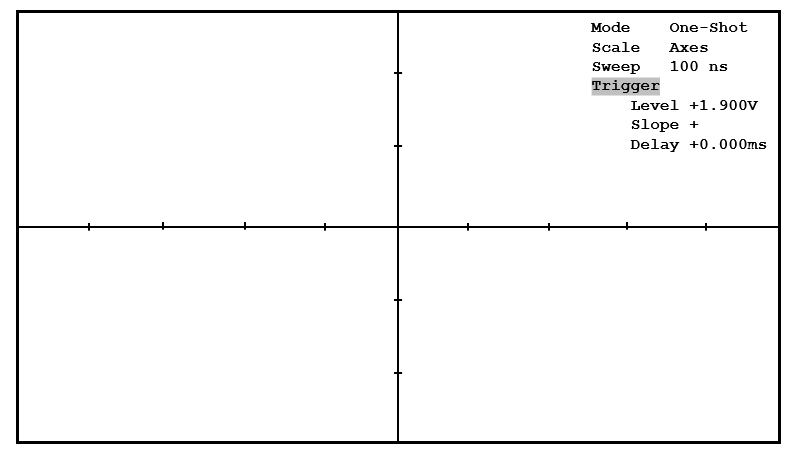
\includegraphics[width=1\textwidth]{{data/Display.png}}
	\caption{Image of display while oscilloscope is on.} 
	\label{Display}    
\end{fullfigure}

\subsection{System Settings}\label{subsec:SystemSettings}

% ADD MENU PICS
\subsubsection{Menu}\index{Menu}
The scope parameter menu is located in the upper right corner of the LCD and contains the following entries in order:

\begin{verbatim}
Mode
Scale
Sweep
Trigger
    Level
    Slope
    Delay
\end{verbatim}

The menu display can be toggled on and off by pressing the menu rotary encoder. The user can cursor to any of the entries by turning the menu rotary encoder and can change a setting by turning the secondary rotary encoder. Changes take effect immediately. More rotary details can be found in section~\ref{subsubsec:RotaryEncoderFunctionality}. The menu entries are described in more detail below.

\begin{description}
	\index{Menu!Mode}\item[Mode]The Mode menu entry can be set to Mode Normal, Mode Automatic, or Mode One-Shot. In Mode Normal the scope waits for another trigger after every retrace. In this mode, new traces are captured as fast as the scope can redraw the screen. Mode Automatic works the same as Mode Normal if there are trigger events. But if no trigger event occurs after a specified delay (typically significantly longer than the time represented by a screen of data) the scope triggers automatically without a trigger event occurring. In Mode One-Shot the scope triggers only once and then holds that trace on the screen. It does not look for another trigger event until the Trigger menu item is selected and secondary rotary encoder is turned.
	
	\index{Menu!Scale}\item[Scale] The Scale menu entry can be set to Scale Axes, Scale Grid, or Scale Off. If the scale is set to Scale Axes, the x and y axes are displayed along with the trace. If the scale is set to Scale Grid, an x-y grid is displayed along with the trace. If the scale is set to Scale Off, no axes or grid are displayed.
	
	\index{Menu!Sweep}\item[Sweep] The Sweep menu entry sets the sweep rate (in time per sample) for the scope. Possible settings are: 100, 200, and 500 nanoseconds, and 1, 2, 5, 10, 20, 50, 100, 200, and 500 microseconds, and 1, 2, 5, 10, and 20 milliseconds (per sample).
	
	\index{Menu!Trigger}\item[Trigger] The Trigger menu entry re-arms the trigger for the scope in one-shot mode. Any time it is selected and the secondary rotary encoder is turned the scope trigger is re-armed and a new trace will then be captured once the trigger conditions (level and slope) are met.
	
	\index{Menu!Level}\item[Level] The Level menu entry sets the trigger level. It can be set to any value from the most negative input voltage to the most positive in 128 steps. Additionally, the trigger level is displayed as a line on the screen when the trigger level is being changed.
	
	\index{Menu!Slope}\item[Slope] The Slope menu entry is either Slope + or Slope - and determines whether the scope is triggered on a positive or negative slope respectively.
	
	\index{Menu!Delay}\item[Delay] The Delay menu entry determines the trigger delay. It sets the time after the trigger event at which the trace will start. It may be set to any value from the minimum delay to the maximum delay times the sample rate and it is displayed as a time.
\end{description}

\subsubsection{Rotary Encoder Functionality} \index{Rotary Encoder Functionality} \label{subsubsec:RotaryEncoderFunctionality}

\begin{fullfigure} 
	\centering
	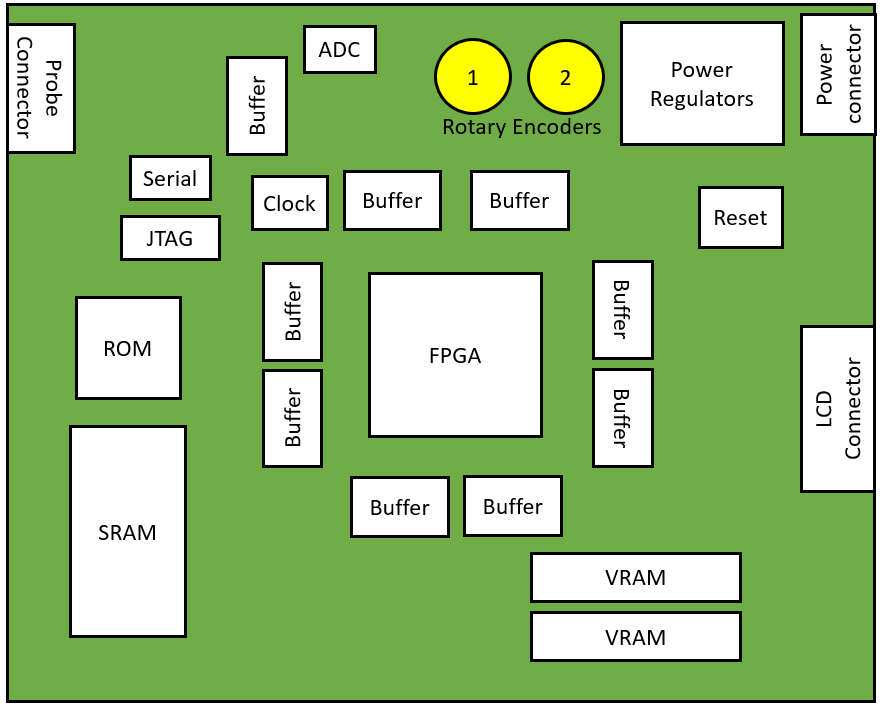
\includegraphics[width=1\textwidth]{{data/Board_Layout_Rotary_Labeled.png}}
	\caption{Board Layout: Labeled Rotary Encoders.} 
	\label{Layout:RotaryLabeled}    
\end{fullfigure}

The user can change the scope configuration via two rotary encoders (seen in Figure~\ref{Layout:RotaryLabeled}). All of the scope parameters are set via an on-screen menu. The rotary actions are detailed below: 
\begin{description}
	\item[Press encoder 1] Turns the menu on/off. If the menu is off it is not displayed and turning the rotary encoders have no effect on the settings.
	
	\item[Turn encoder 1 CW] Moves the cursor down, if not already at the bottom menu item. If at the bottom, the cursor does not move. 
	
	\item[Turn encoder 1 CCW] Moves the cursor up, if not already at the top menu item. If at the top, the cursor does not move.
	
	\item[Turn encoder 2 CW] Changes the currently selected (with cursor) menu item. Goes "forward" through the list of possible settings. If at the "end" of the list, doesn't change the current selection.
	
	\item[Turn encoder 2 CCW] Changes the currently selected (with cursor) menu item. Goes "backward" through the list of possible settings. If at the "beginning" of the list, doesn't change the current selection.
\end{description}

%IS THERE ANYTHING ELSE? IDK 

\section{Technical Documentation} 
\subsection{Hardware} 
\subsubsection{Hardware System Overview} 
\begin{comment}
			System overview 
	Very high level description
	Use block diagram 
	Describe how the system works and how blocks interact 
	Easiest to describe in terms of UI interactions 
	Can be multi-level (may not need that much detail at system level) 
	Ex: how signal moves through scope to get to display 
	1-2 pages of text
\end{comment}
% BLOCK DIAGRAM
\begin{fullfigure} 
	\centering
	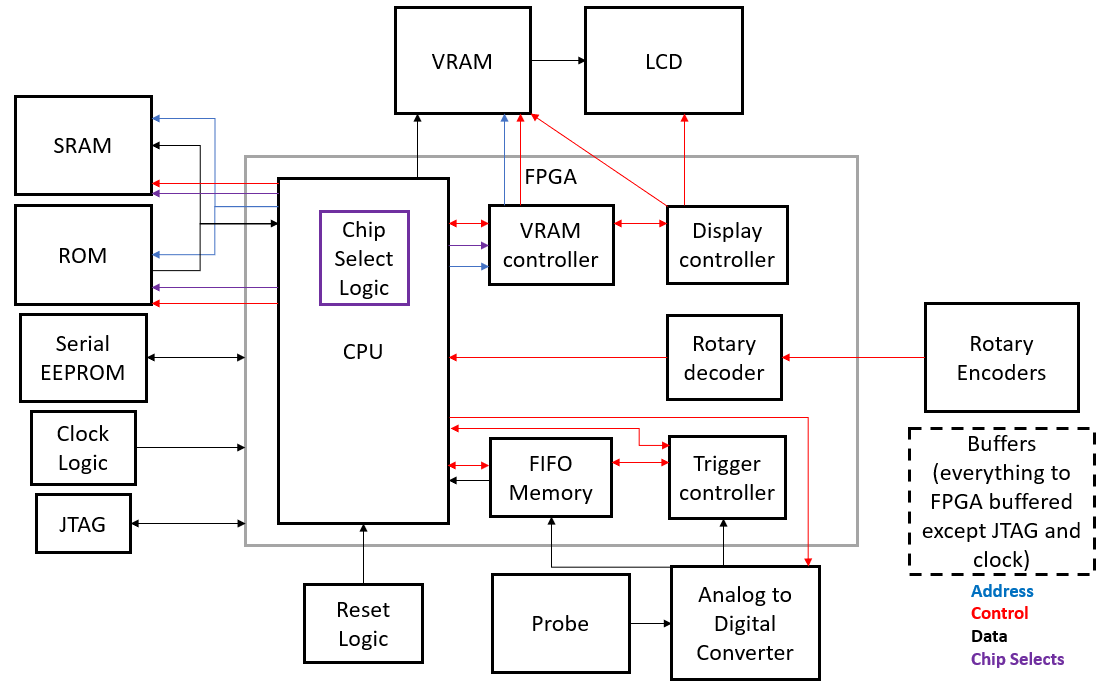
\includegraphics[width=1\textwidth]{{data/blockmain.png}}
	\caption{Block diagram overview of FPGA and peripheral chips.} 
	\label{Block:main}    
\end{fullfigure}
% BOARD LAYOUT
\begin{fullfigure} 
	\centering
	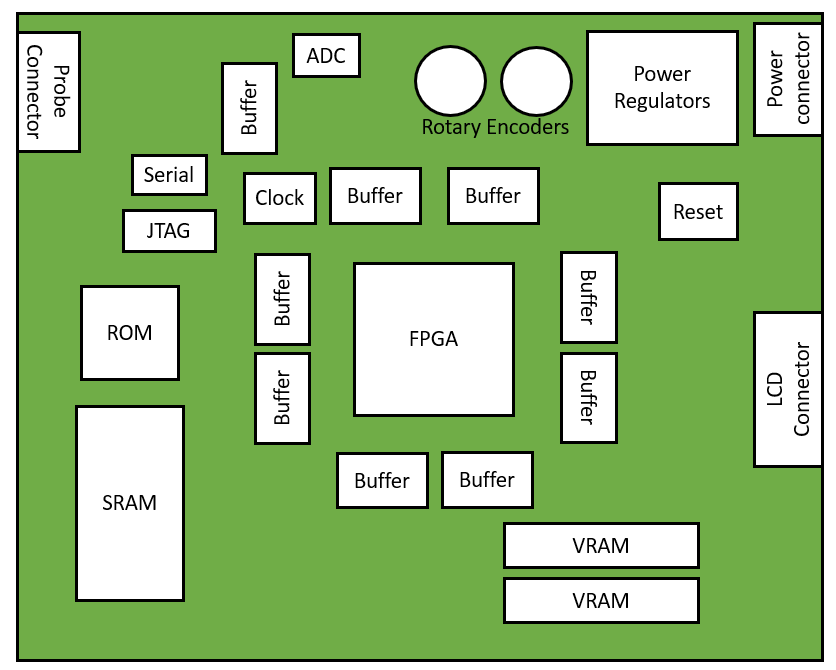
\includegraphics[width=1\textwidth]{{data/Board_Layout.png}}
	\caption{Board Layout.} 
	\label{Layout:main}    
\end{fullfigure}

\begin{fullfigure} 
	\centering
	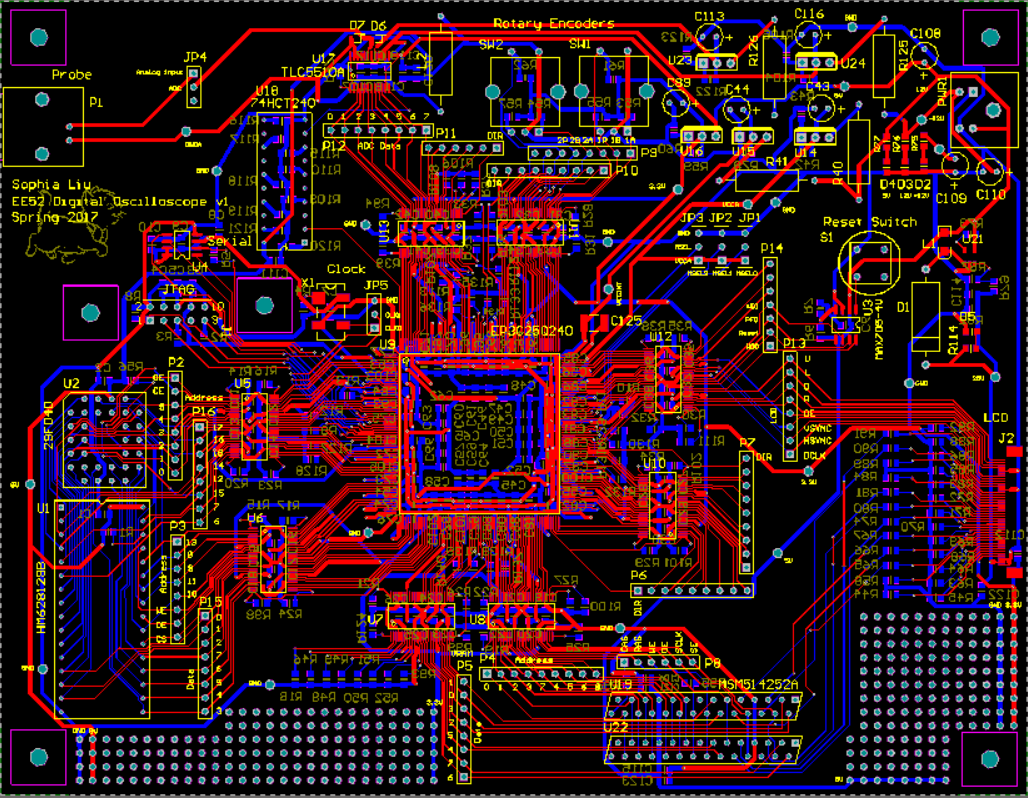
\includegraphics[width=1\textwidth]{{data/PCB.png}}
	\caption{Image of PCB.} 
	\label{PCB}    
\end{fullfigure}

% MEMORY MAP
The oscilloscope system is centered around a Cyclone III FPGA, which includes a Nios II CPU and controllers for the VRAM, LCD, rotary encoders, and analog input and triggering. Upon startup, the bitmap %TODO is it a bitmap???
is loaded from the serial EEPROM. The %SOFTWARE? 
is then loaded from the ROM.

\marginlabel{Receiving a Signal:} When the probe is connected to a desired input, the analog signal is sent to an Analog to Digital Converter chip. 8 bits of data are then sent in parallel to the FPGA to an analog controller. The various trigger setting inputs (auto triggering, trigger enable, trigger slope, trigger level) are used along with the 8 bit signal to determine if the system should begin sampling. Once triggering has occurred, the signal is written to a %SIZE, 512 
FIFO buffer at the sampling rate. Once the FIFO is full, the CPU clocks out and stores the buffer data to be displayed. 

\marginlabel{Displaying a Signal:} In order to display the signal on the LCD, data is written to the VRAM, which is then sent out to the LCD. Several control signals (write enable, chip select, address, wait) are sent from the CPU to the VRAM controller to perform read and write operations on the VRAM. An LCD controller sends out the necessary control signals to display the signal. 

% the other things 

\subsubsection{FPGA} \index{FPGA}%HERE? idk. talk about controllers 
\begin{fullfigure} 
	\centering
	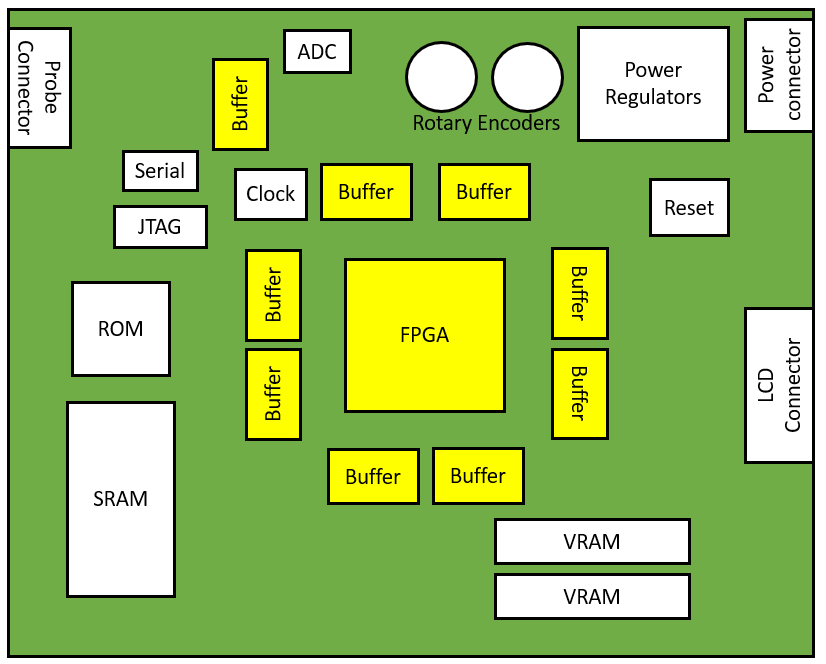
\includegraphics[width=1\textwidth]{{data/Board_Layout_FPGA.png}}
	\caption{Board Layout: FPGA and buffers.} 
	\label{Layout:FPGA}    
\end{fullfigure}

An Altera Cyclone III FPGA was used for all the logic and processing required (U9, EP3C25Q240). The three required voltage levels were generated with regulators, and each power pin was locally bypassed. The full schematics with the FPGA can be seen in Appendix~\ref{AP:Schematics}.

%level shifters / buffers 
Buffers, or level shifters, were used to connect the buses and control signals from the peripheral chips to the FPGA to go between the low FPGA voltage and mainly 5V environment (U5, U6, U7, U8, U10, U12; 74LVT16245). A separate buffer was used to interface with the ADC (U17, TLC5510A), which had a larger input voltage range requirement (U18, SN74HCT240).

% pinout 
\marginlabel{Pin Assignments:} The pins were connected on the PCB as listed below. 
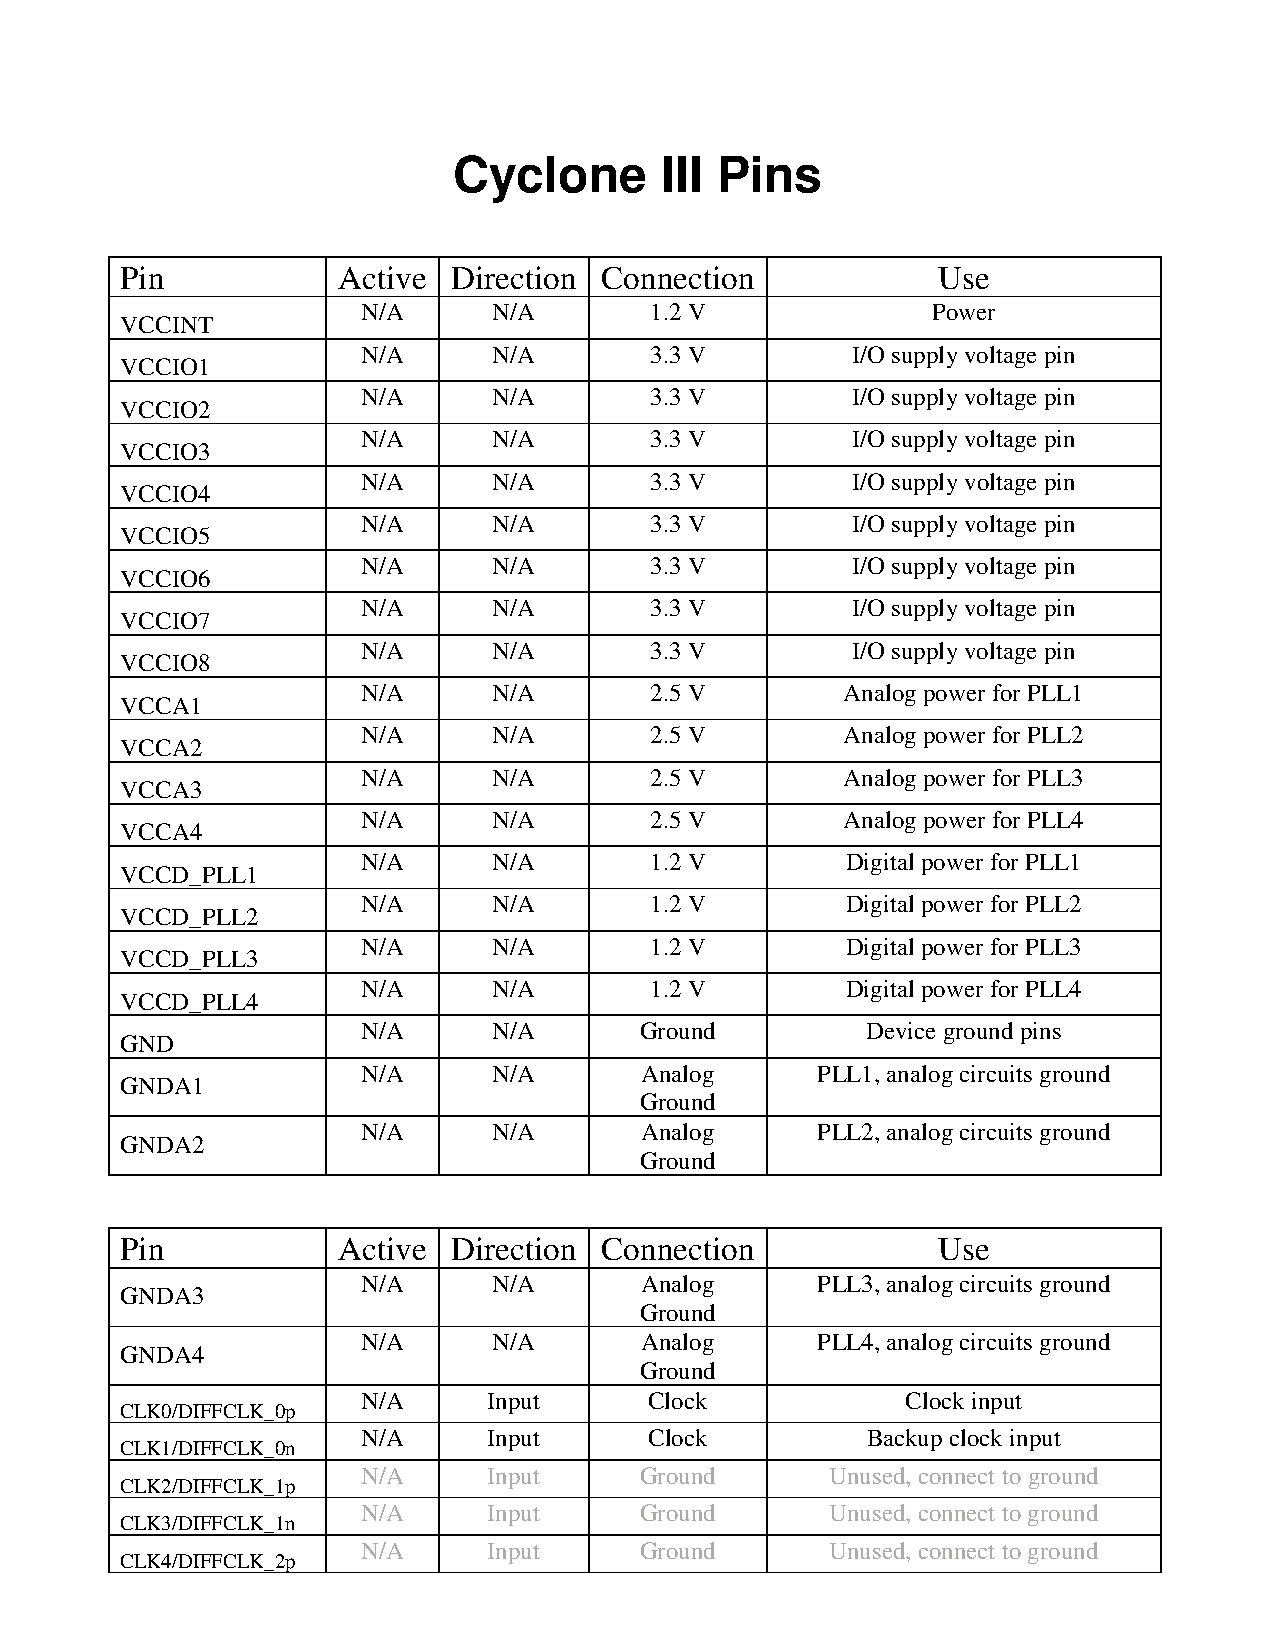
\includepdf[pages={-}]{data/Cyc3Pins.pdf} 

The final product included several changes. Pin 162, an output for device configuration, was left floating, and the reset input was changed to Pin 187. One buffer was also left unusable, resulting in rewiring to extra I/O pins. The pin assignments are shown below.  
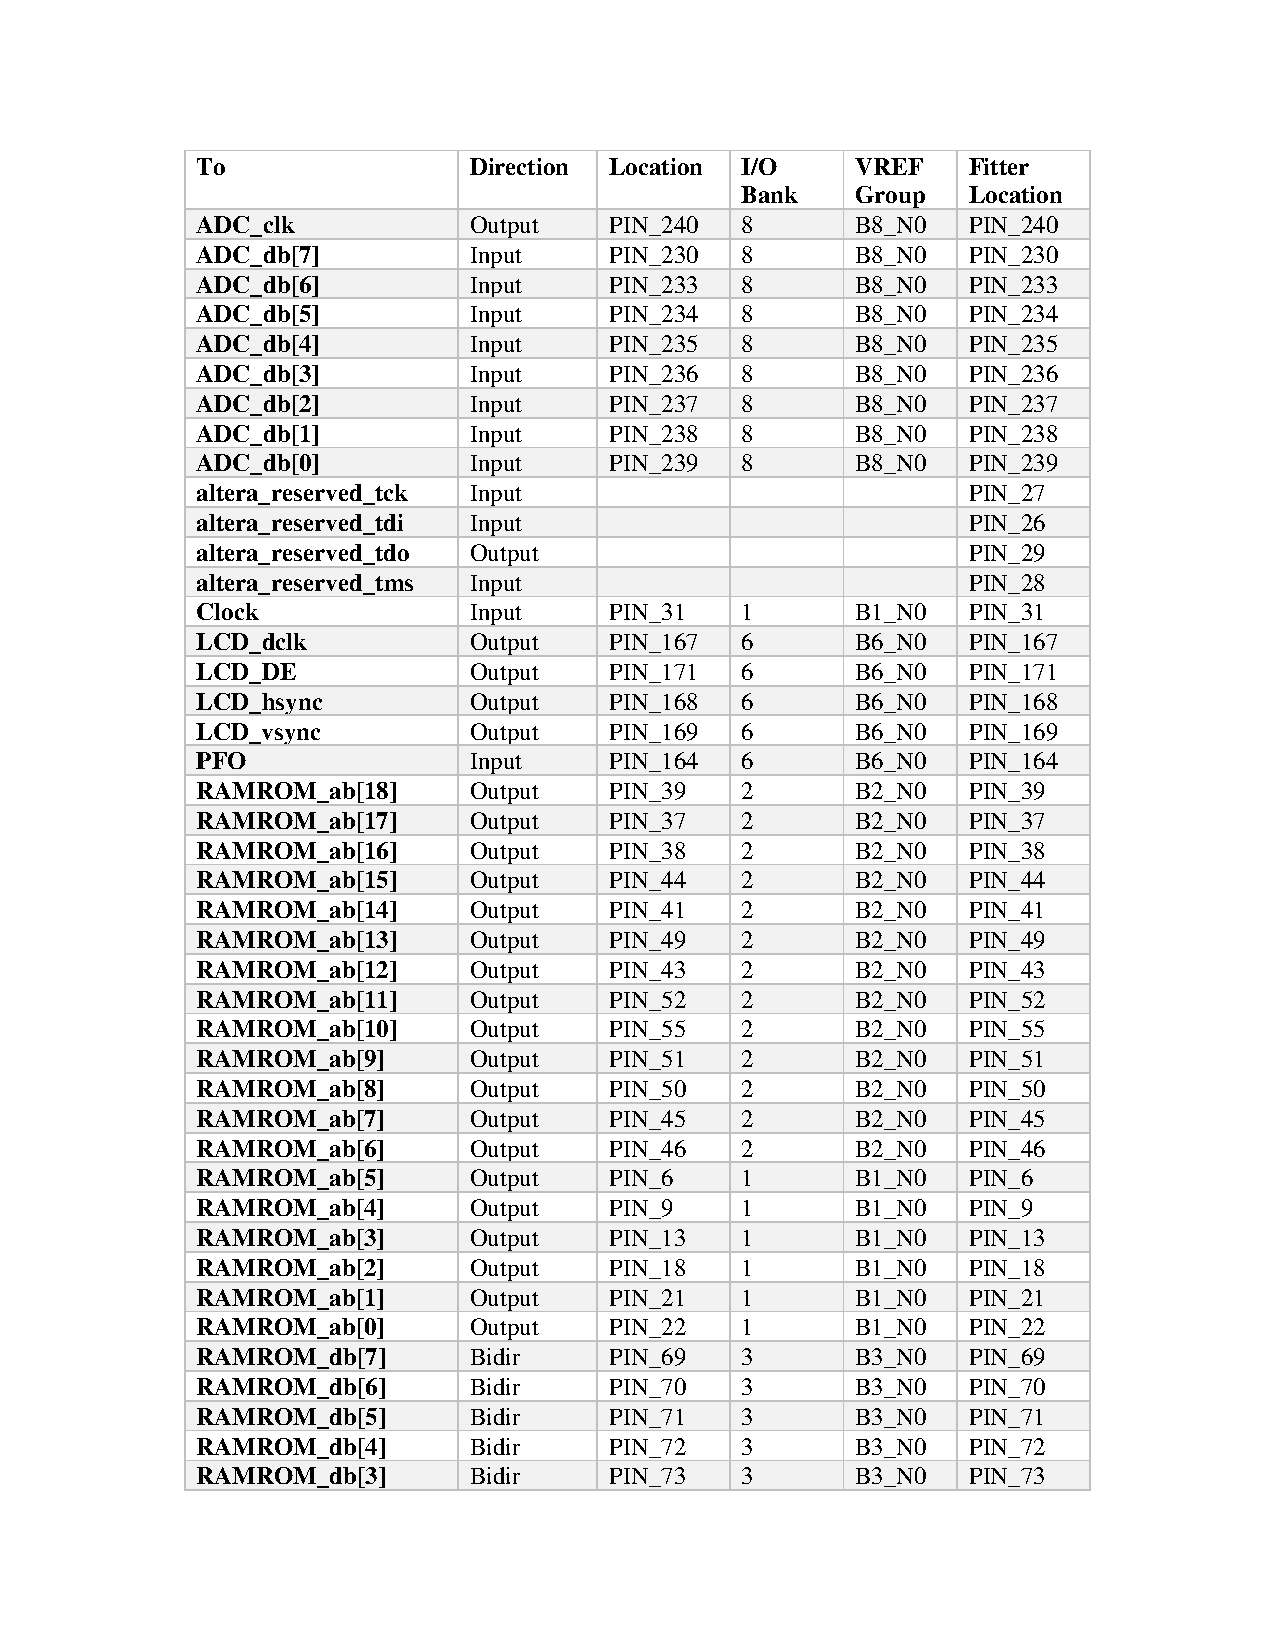
\includepdf[pages={-}]{data/Cyc3Pins_final.pdf} 

% block diagram
\begin{fullfigure} 
	\centering
	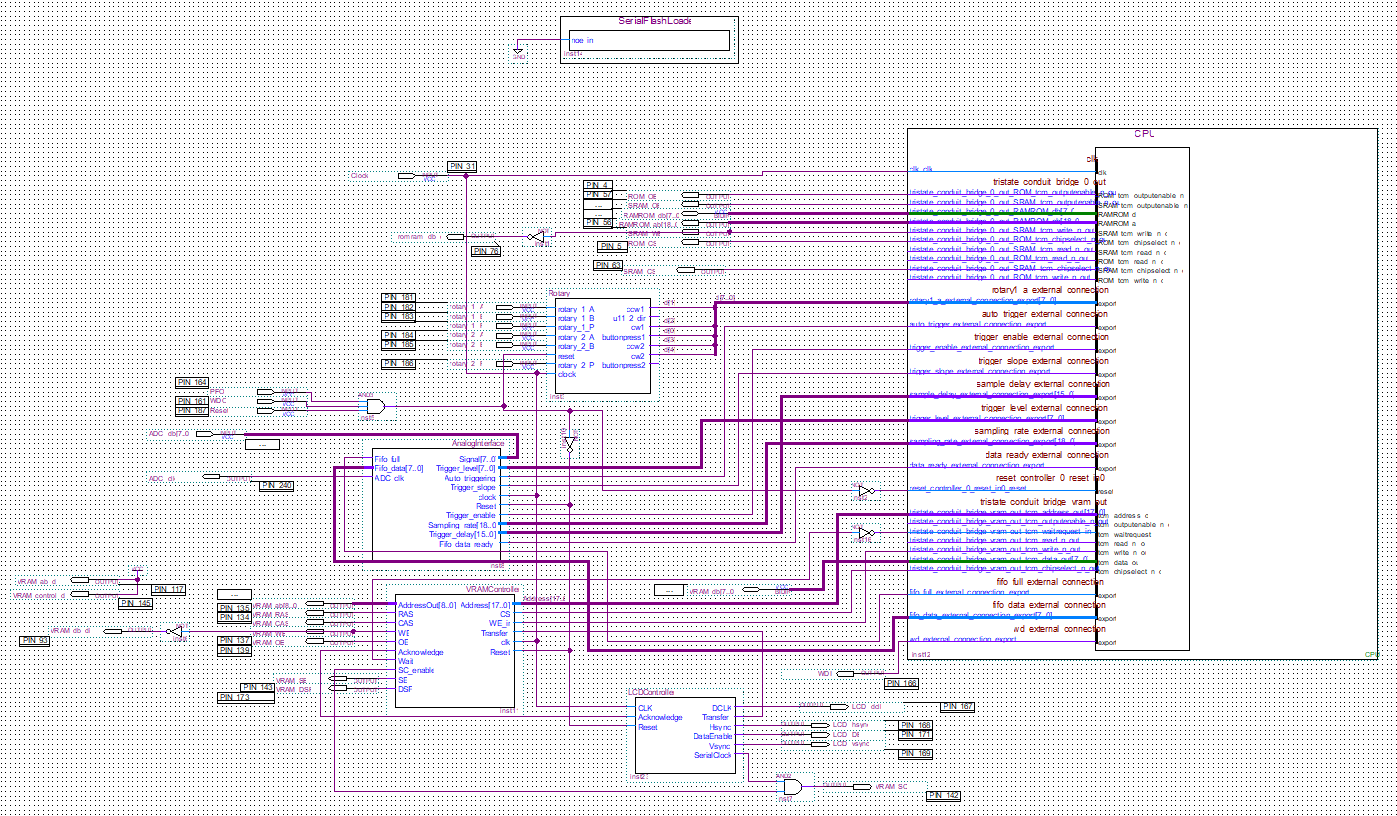
\includegraphics[width=1\textwidth]{{data/CPU.png}}
	\caption{The main FPGA block diagram with the CPU, inputs and outputs, and controllers.} 
	\label{Block:CPU}    
\end{fullfigure}

%logic 
\marginlabel{Logic:} A CPU and several controllers were programmed into the FPGA, as seen in Figure~\ref{Block:main}. These will be discussed in greater detail in their respective subsections. As seen in the main block diagram, the peripheral memory, user interface elements, and other elements all interact with the FPGA and its various controllers. The input signal and settings are sent to the CPU and the appropriate controllers, and the output data is sent from the CPU to be displayed on the LCD.

%TODO more??

\subsubsection{Power} \index{Power} \label{subsec:Power}

\begin{fullfigure} 
	\centering
	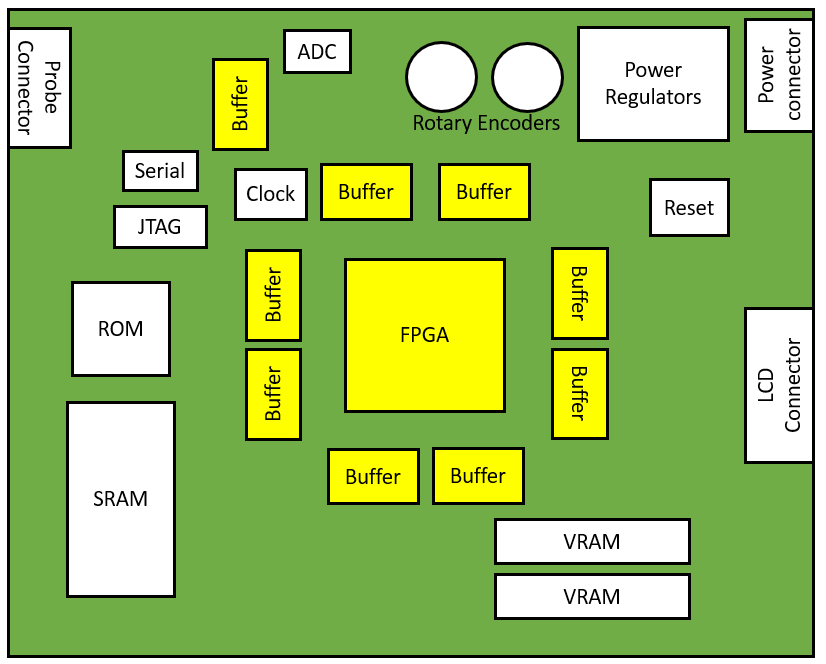
\includegraphics[width=1\textwidth]{{data/Board_Layout_FPGA.png}}
	\caption{Board Layout: Power circuitry.} 
	\label{Layout:Power}    
\end{fullfigure}
The full power schematics can be found at Appendix~\ref{AP:Schematics}.

A din4 connector (PWR1) is used to supply the board with +/-12 V and 5 V. All chips are locally bypassed.

5 V is used to power the reset, VRAM, SRAM, ROM, and ADC chips. 
Several LM1086 regulators are used to generate the other required voltages. Specifically, U14 uses the 5 V supply to generate 2.5 V for analog power to the FPGA PLLs, and U15 uses the 5 V supply to generate 1.2 V for FPGA power supply and digital power to the FPGA PLLs. U16 generates 3.3 V from 5 V, which is used to power the FPGA I/O supply pins, buffers, JTAG, serial configuration device, clock, and for pulling high the rotary encoder outputs.

Regulators also generate 5 V from 12 V (U24) and 4 V from 5 V (U23) for ADC reference voltages. The main power schematics can be seen in Figure~\ref{}.

A boost converter is used to generate the 25 V necessary for the LCD backlight. U21 (AP3012) steps up from 5 V and outputs 25 V  (Figure~\ref{Schematic:LCDpower}).

% boost converter 
\begin{fullfigure} 
	\centering
	\includegraphics[width=0.9\textwidth]{{data/LCD_power.png}}
	\caption{Boost converter circuit for LCD backlight power supply.} 
	\label{Schematic:LCDpower}    
\end{fullfigure}

\subsubsection{Memory} \index{memory} \label{subsec:Memory}

\begin{fullfigure} 
	\centering
	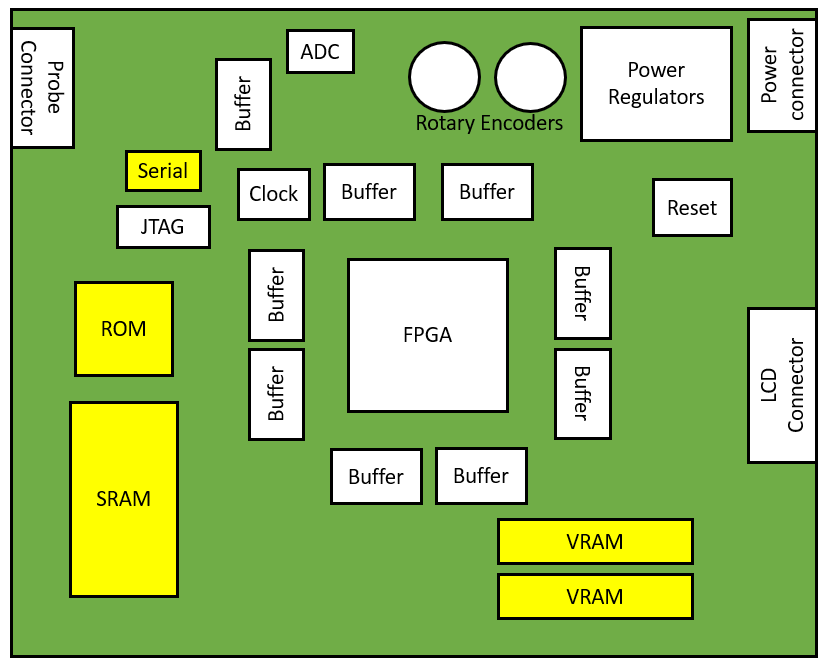
\includegraphics[width=1\textwidth]{{data/Board_Layout_Memory.png}}
	\caption{Board Layout: Memory.} 
	\label{Layout:Memory}    
\end{fullfigure}

\marginlabel{Memory Map:} 
%TODO explain? 
\begin{fullfigure} 
	\centering
	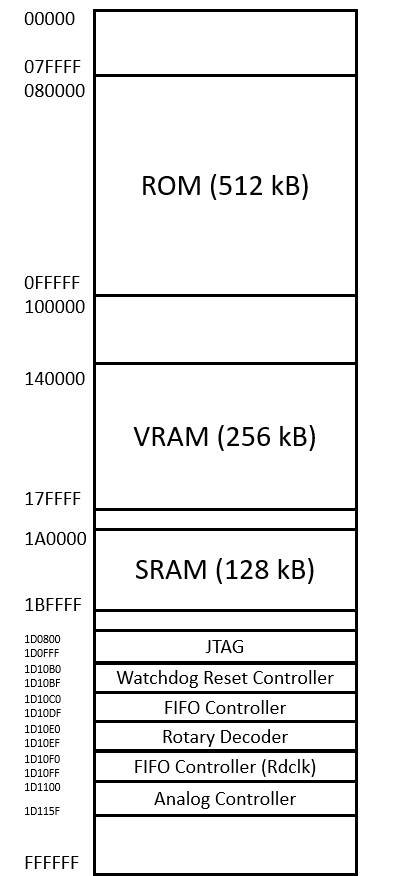
\includegraphics[width=0.4\textwidth]{{data/memorymap.png}}
	\caption{Memory map diagram} %used by the CPU(?)
	\label{Block:Memorymap}    
\end{fullfigure}

Several types of storage were used, including ROM (U2) for permanent program storage, and a smaller amount of static RAM (U1) for storage including the data segment, stack, and heap. Video RAM (U19, U22), with dynamic RAM, which is cheaper and smaller than static RAM, and serial memory, was used for the display memory. A serial device (U4) was also used to store configuration data for the FPGA after powering on. 

\marginlabel{ROM:} \index{ROM}
1 512 K x 8 bit EEROM (U2, Am29F040) was used for program storage. %correct tense hell
8 data bits are connected in parallel through the buffers to the CPU, along with 19 address bits, an active-low chip enable (CE), and output enable (OE) signal. The write enable (WE) signal was pulled up, as the ROM was written to with a dedicated ROM programmer.

The ROM timing diagram for the read cycle can be seen at Appendix~\ref{AP:Timing}, Figure~\ref{AP:ROM_Read_Timing}. 3 read wait states were used. %is this the right way to say it?

The executable file from the Nios II IDE was loaded into the ROM using a ROM programmer. 

\begin{fullfigure} 
	\centering
	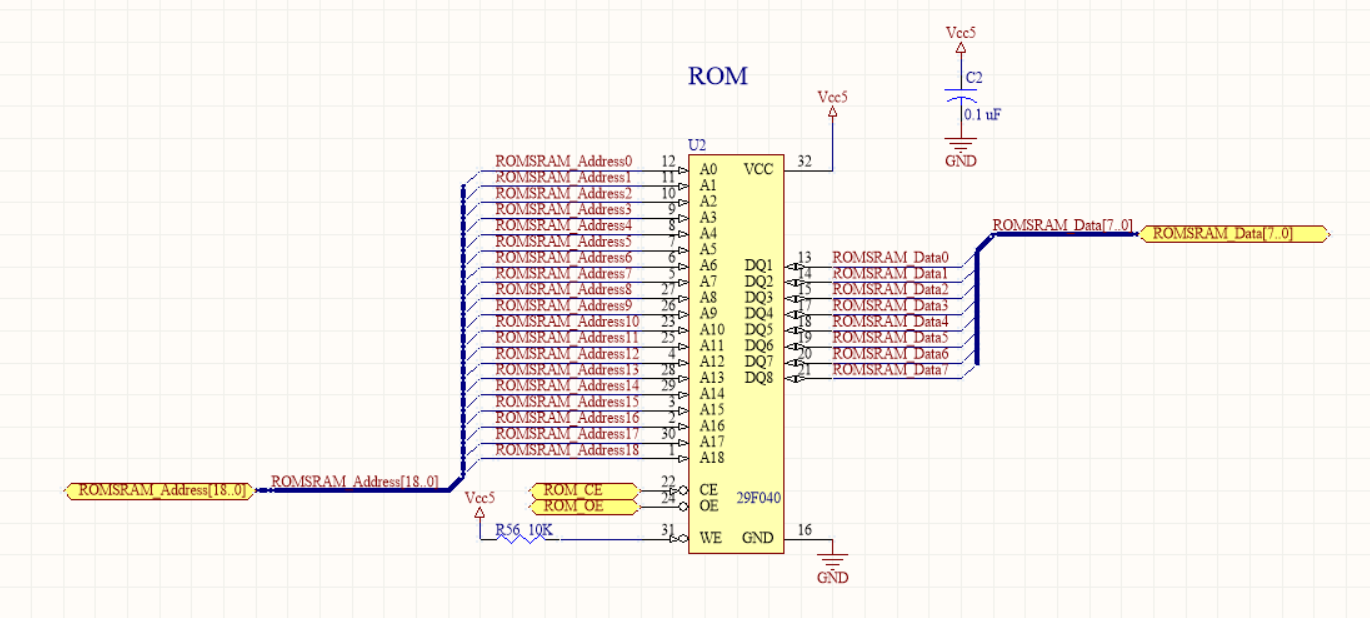
\includegraphics[width=1\textwidth]{{data/ROM.png}}
	\caption{ROM Schematic.}
	\label{Schematic:ROM}    
\end{fullfigure}

%block diagram

\marginlabel{SRAM:} \index{SRAM}
1 128 K x 8 bit CMOS static RAM was used (U1, HM628128B) 

The address line is shared between the ROM and SRAM, with only the 17 least significant bits used for RAM addressing. The 8-bit data bus is also shared between the ROM and SRAM. The active-low output enable (OE), write enable (WE), and chip select (CS1) are also connected between the SRAM and CPU, with the second active high chip select (CS2) pulled high as required by the read and write cycles. 

The SRAM timing diagrams can be seen at Appendix~\ref{AP:Timing},
Figures~\ref{AP:RAM_Read_Timing} and \ref{AP:RAM_Write_Timing}. 2 read wait states and 1 write wait state was used. 

\begin{fullfigure} 
	\centering
	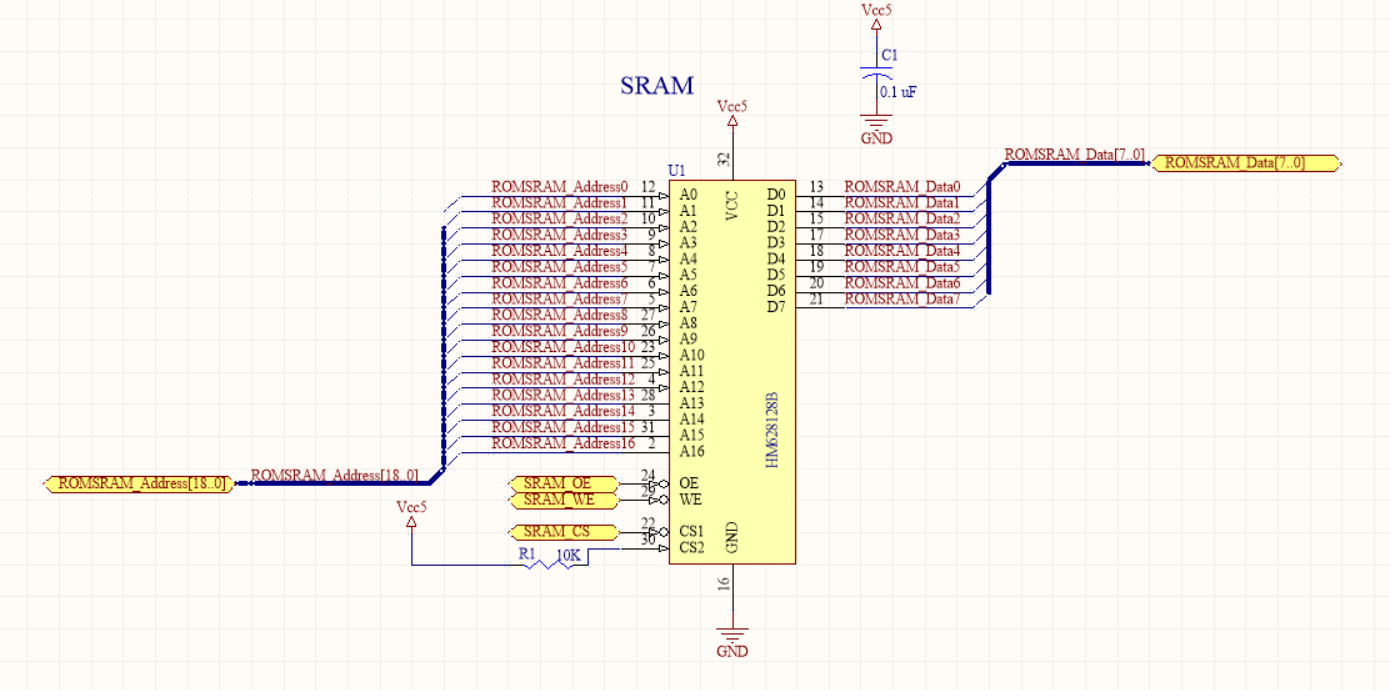
\includegraphics[width=1\textwidth]{{data/SRAM.png}}
	\caption{SRAM Schematic.}
	\label{Schematic:SRAM}    
\end{fullfigure}

\marginlabel{VRAM:} See Section~\ref{subsec:VRAMLCD} for details on the VRAM.
 
\marginlabel{Serial Device:} \index{Serial Device}
A serial configuration device (U4, EPCS16), a 2 MB flash memory device, was used to store FPGA configuration data \footnote{Was unable to successfully use serial device for unknown reasons, possibly due to incorrect FPGA configurations.}.

\begin{fullfigure} 
	\centering
	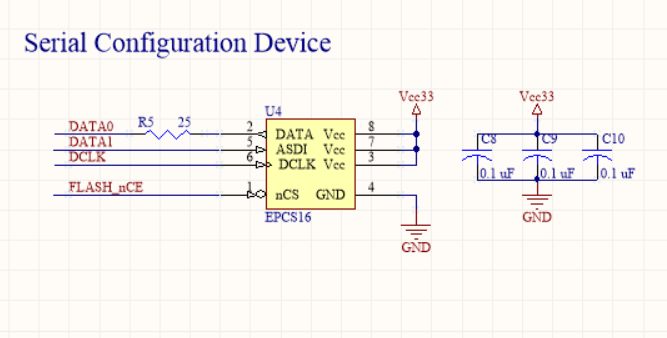
\includegraphics[width=0.75\textwidth]{{data/EEPROM.png}}
	\caption{Serial Device Schematic.}
	\label{Schematic:EEPROM}    
\end{fullfigure}

\subsubsection{Analog System}\index{Analog!Hardware} \label{subsec:AnalogHardware}
\begin{fullfigure} 
	\centering
	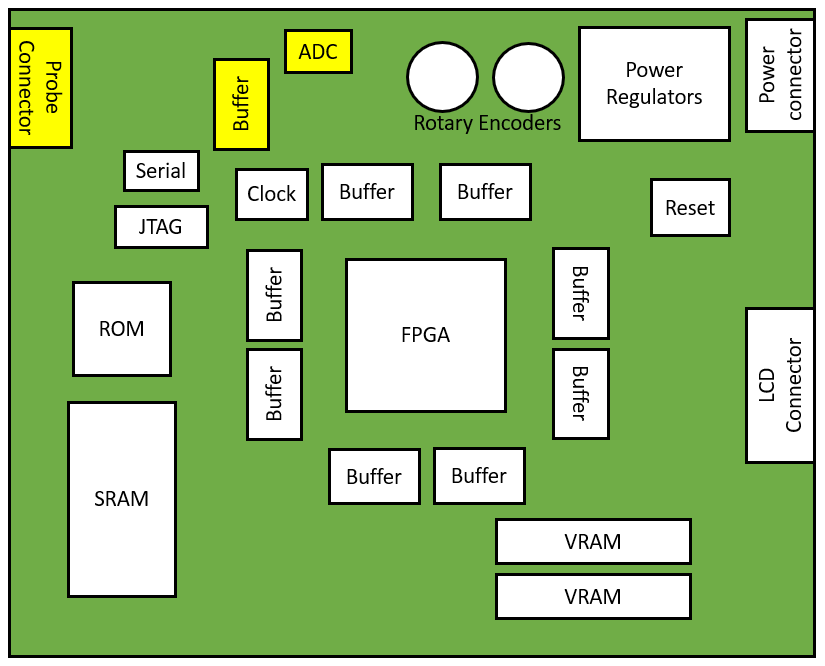
\includegraphics[width=1\textwidth]{{data/Board_Layout_ADC.png}}
	\caption{Board Layout: Analog circuitry.} 
	\label{Layout:Analog}    
\end{fullfigure}

% schematics
\begin{fullfigure} 
	\centering
	\includegraphics[width=1\textwidth]{{data/ADC.png}}
	\caption{ADC circuit schematic.} 
	\label{Schematic:ADC}    
\end{fullfigure}

\begin{fullfigure} 
	\centering
	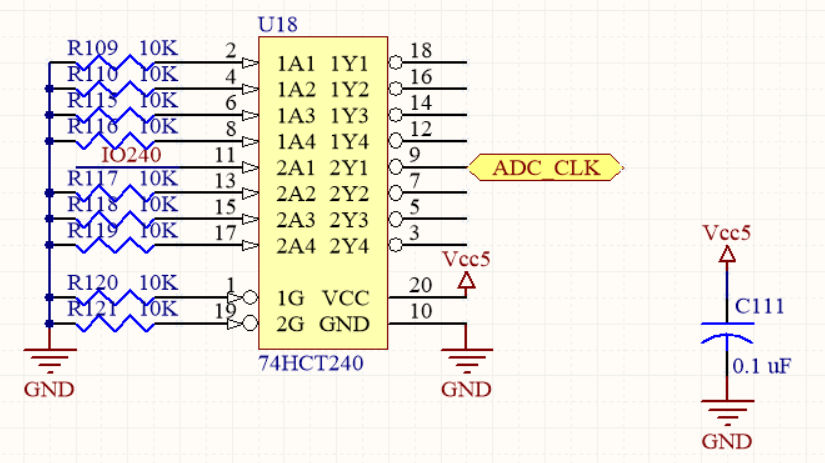
\includegraphics[width=0.8\textwidth]{{data/ADC_Buffer.png}}
	\caption{Buffer for FPGA to ADC signals.} 
	\label{Schematic:ADC_Buffer}    
\end{fullfigure}

% summary 
\marginlabel{Summary:} An analog signal is inputted through the BNC connector (P1). A jumper connector was used in case additional analog front end circuitry was used. The signal then passes through protection diodes and is sent to the ADC. The data is then sent through the buffers to the FPGA and analog controller, which stores the signal at the sampling rate once it has been triggered.

% design decisions?
\marginlabel{ADC:} The analog input can range from 0 to 4 V. An analog-to-digital converter (U17, TLC5510A) was used to digitize the input signal to 8 bits. This specific ADC was chosen because of the simplicity of the circuit needed in order to meet the 0-3 V requirement.

% pins 
The 8 bit data bus was connected to the CPU in parallel, and a clock input was generated from the analog controller. A separate buffer was required to meet the ADC input voltage requirements (U18 in Figure~\ref{Schematic:ADC_Buffer}). Protection diodes (D6, D7 in Figure~\ref{Schematic:ADC}) with a low forward voltage (about 0.2 V) were used to keep the analog input within the allowed input range. 

Several analog supply voltages were used to isolate the analog and digital circuitry. An external 4 V analog reference was generated and used for a 0-4 V input signal range. A 5 V analog power supply was also required, along with an analog ground reference connected to digital ground through a power inductor (Part L2, Figure~\ref{}). 

\marginlabel{Analog logic:}
\index{Analog!Logic}
The analog controller consists of a trigger controller to determine when a trigger has occurred, along with logic for storing the signal at the specified sampling rate. If a trigger occurs, or if the auto triggering times out, the signal is stored in a FIFO buffer to be clocked out and displayed. 

% block diagram
\begin{fullfigure} 
	\centering
	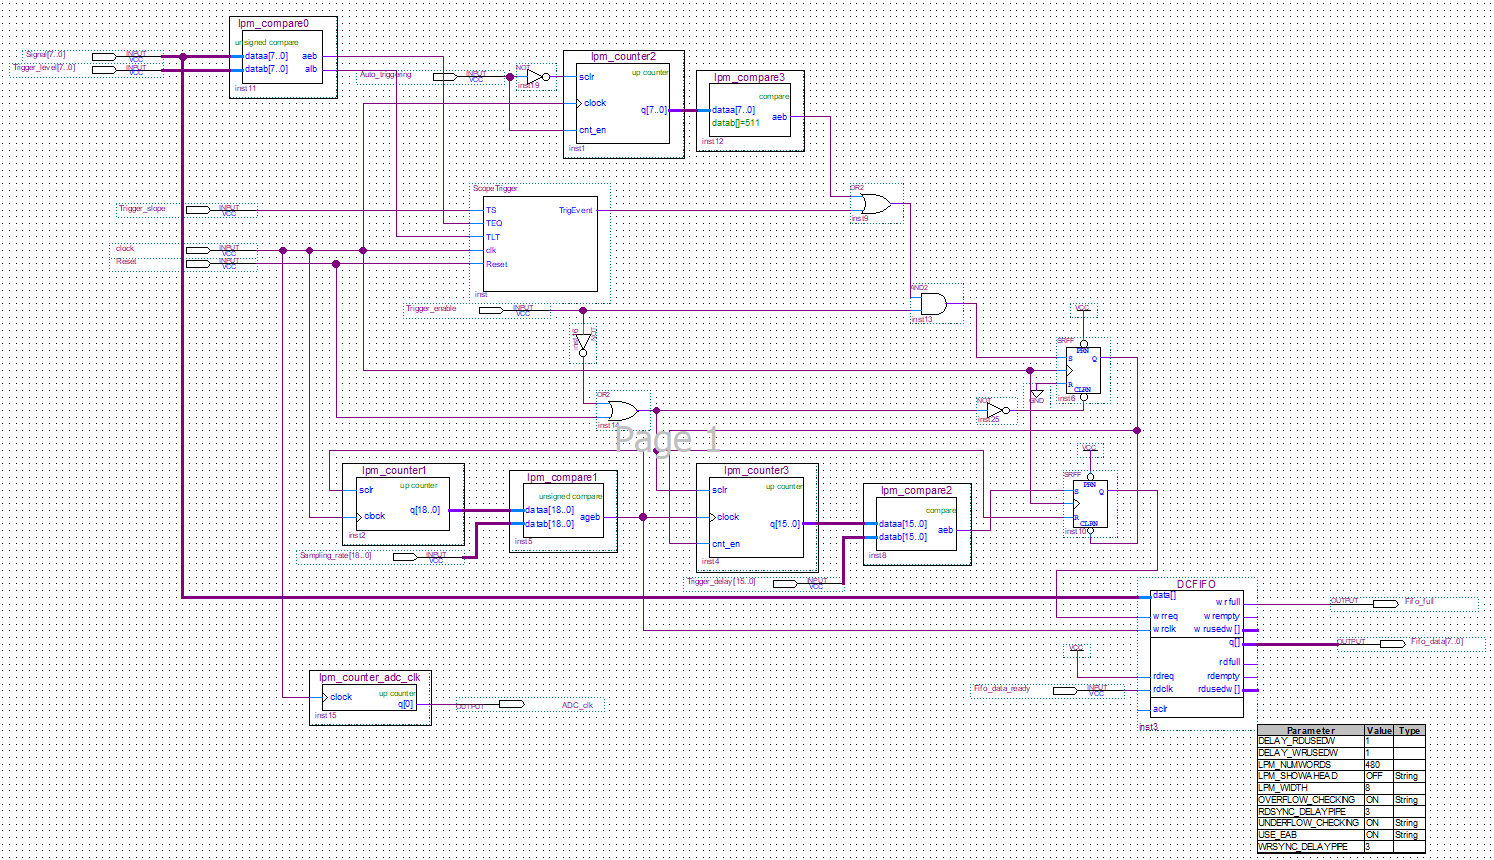
\includegraphics[width=1\textwidth]{{data/Analog_Controller.png}}
	\caption{Analog controller block diagram.} 
	\label{Block:Analog}    
\end{fullfigure}

\marginlabel{Analog input settings:}
Several values are taken as outputs from the CPU and are used in the hardware logic. Specifically, an 8 bit trigger level, 1 bit auto triggering, 1 bit trigger slope, 1 bit trigger enable, 19 bit sampling rate, and 16 bit trigger delay signal are used as set by the user. 

\marginlabel{Trigger logic:} \index{Trigger}
First, the system determines whether or not a trigger has occurred.
A Moore state machine (the ScopeTrigger block in Figure~\ref{Block:Analog}) is used to determine whether or not a trigger has occurred. The trigger event output is set high when the trigger slope is positive and the signal has transitioned from below to above the trigger level, or if the trigger slope is negative and the signal has transitioned from above to below the trigger level. The logic description can be found at Appendix~\ref{scopetrig.vhd}.

In order to do this, the 8-bit signal is compared to the trigger level in lpm\_compare0 in Figure~\ref{Block:Analog}, and the outputs are sent to the trigger state machine.

\index{Trigger!Autotrigger} 
\marginlabel{Autotriggering:} The system also generates a trigger event after 512 clocks if auto trigger is enabled, which was arbitrarily chosen as a short amount of time. Future designs may be improved by correlating the auto trigger countdown to the number of samples and the sampling rate.

An SRFF is set once a trigger event has occurred, and the controller is reset to wait for another trigger event when the trigger enable signal is disabled and re-enabled (set low then high).  

\marginlabel{FIFO buffer storage:} \index{FIFO} A FIFO buffer is used to store the signal once a trigger event has occurred (DCFIFO in Figure ~\ref{Block:Analog}). The FIFO has a size of 480 (the width of the LCD) x 8 bits of data. Once a trigger event has occurred, a counter and comparator are used to create the trigger delay, and an SRFF is set once the delay has been reached to enable writing to the FIFO. A counter and comparator are used to create a clock at the given sampling rate, which is sent to the write clock of the FIFO. The signal is then written into a FIFO buffer at the sampling rate once the trigger delay has finished, and is clocked out by the CPU when it is full. 

\marginlabel{Analog outputs:} As seen in Figure ~\ref{Block:Analog}, the Fifo\_full signal indicates when the FIFO is full and the sample has been stored, the Fifo\_data bus contains the stored signal data. The Fifo\_data\_ready input is controlled from the CPU, which sends the clock necessary to read out the signal from the data bus.

The ADC clock (ADC\_clk) is also outputted from the controller to the ADC. It is is half the 24 MHz system clock (or a 12 MHz clock) because of the maximum ADC conversion rate, which is 20 M samples per second.

\subsubsection{Rotary Encoders}\index{Rotary Encoders} \label{subsec:Rotary}
\begin{fullfigure} 
	\centering
	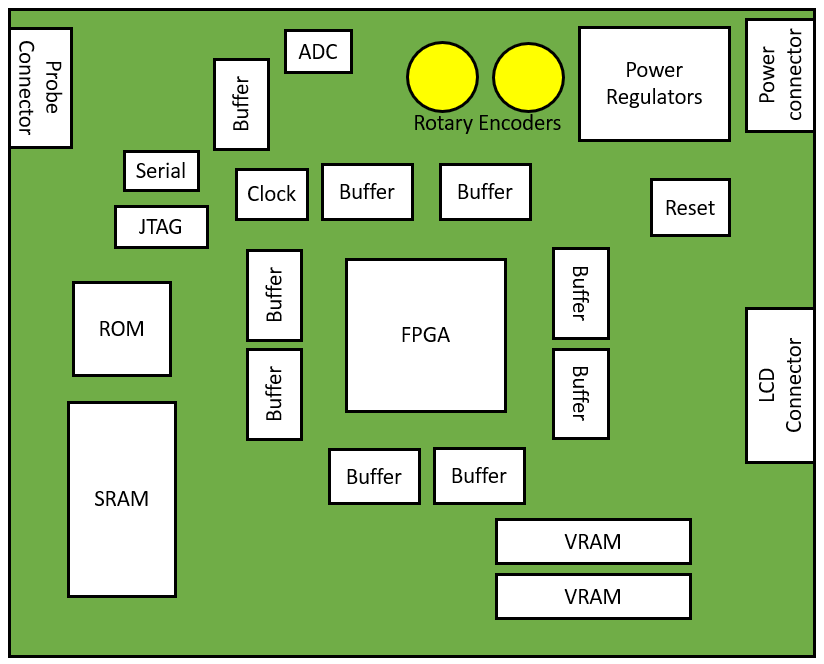
\includegraphics[width=1\textwidth]{{data/Board_Layout_Rotary.png}}
	\caption{Board Layout: Rotary Encoders.} 
	\label{Layout:Rotary}    
\end{fullfigure}

\begin{fullfigure} 
	\centering
	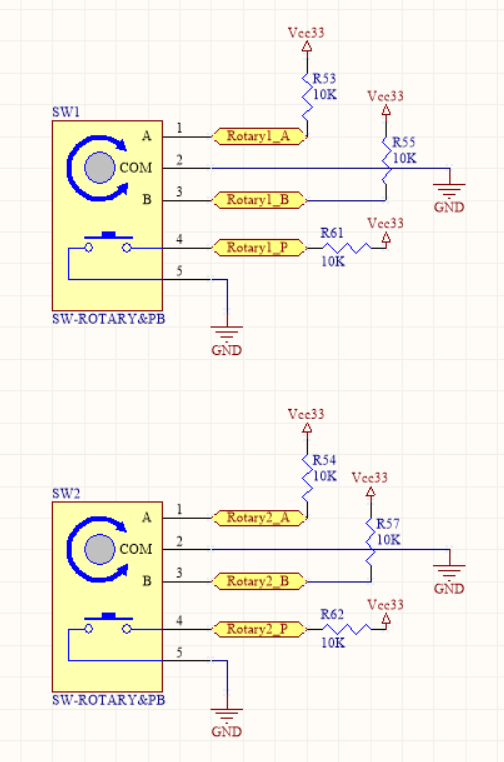
\includegraphics[width=0.5\textwidth]{{data/Rotary.png}}
	\caption{Rotary encoders schematics.} 
	\label{Schematics:Rotary}    
\end{fullfigure}

Two rotary encoders are used for the user input (SW1, SW2).
These include and A and B output for the encoder and a single pull single throw push button switch. 

Pins A and B are pulled high\footnote{1 K resistors were used in place of the 10 K resistors on the schematic because the voltage high output was too low for the buffers.}, while the common pin was grounded to create out-of-phase pulses from outputs A and B.

\marginlabel{Rotary decoder logic:} 
\begin{fullfigure} 
	\centering
	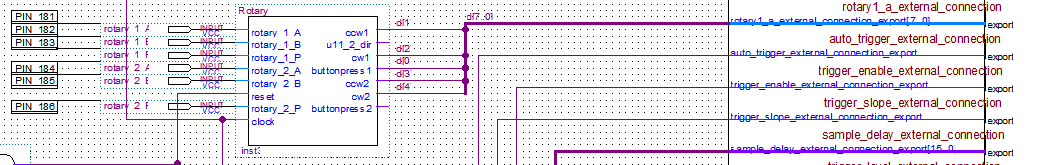
\includegraphics[width=1\textwidth]{{data/RotaryCPU.png}}
	\caption{Connections between CPU and rotary controller.} 
	\label{Block:RotaryCPU}    
\end{fullfigure}

\begin{fullfigure} 
	\centering
	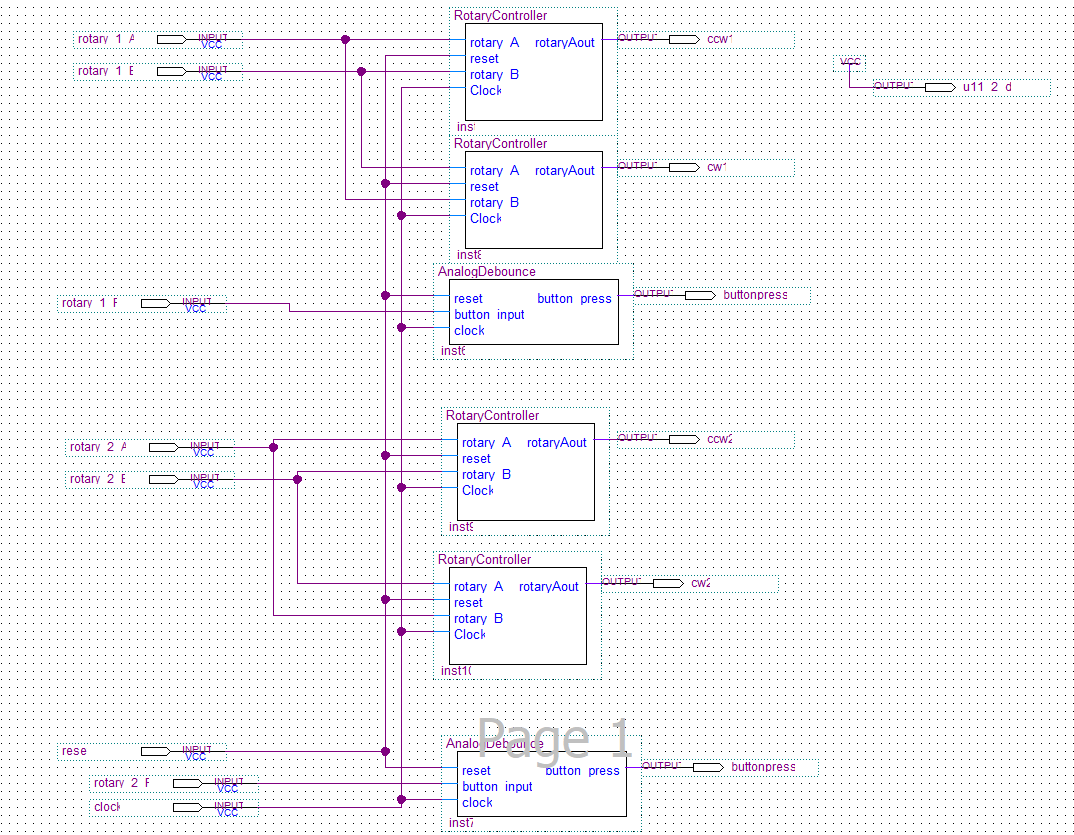
\includegraphics[width=1\textwidth]{{data/RotaryBlock.png}}
	\caption{Rotary controller.} 
	\label{Block:Rotary}    
\end{fullfigure}

\begin{fullfigure} 
	\centering
	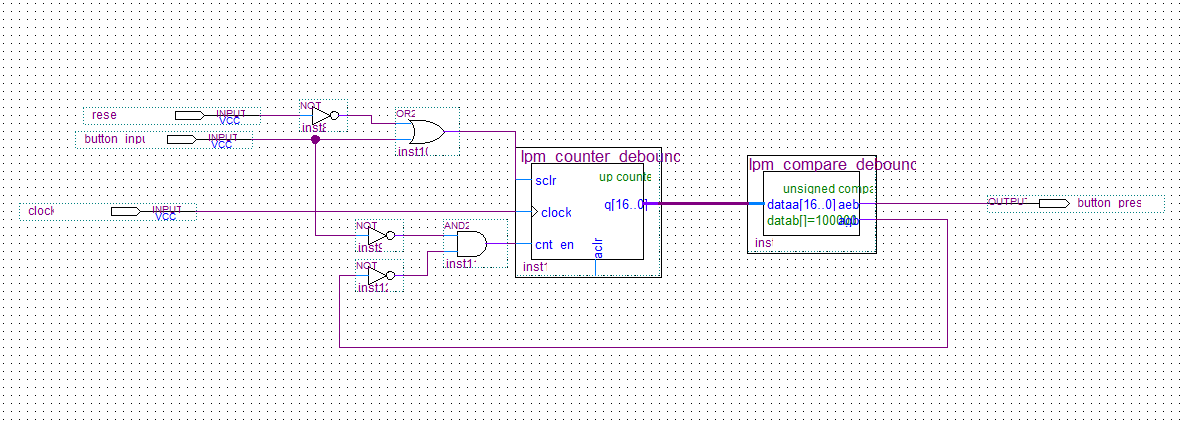
\includegraphics[width=1\textwidth]{{data/Debouncer.png}}
	\caption{Debouncer for push button.} 
	\label{Block:RotaryDebouncer}    
\end{fullfigure}

\begin{fullfigure} 
	\centering
	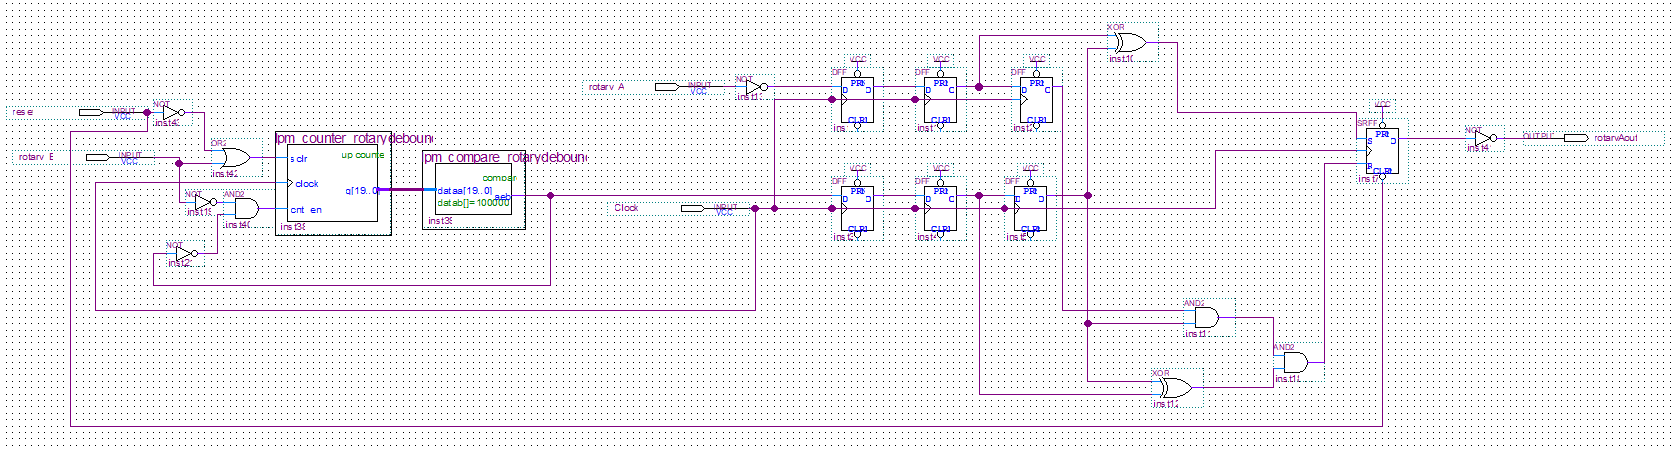
\includegraphics[width=1\textwidth]{{data/RotaryController.png}}
	\caption{Rotary decoder.} 
	\label{Block:RotaryDecoder}    
\end{fullfigure}

\begin{fullfigure} 
	\centering
	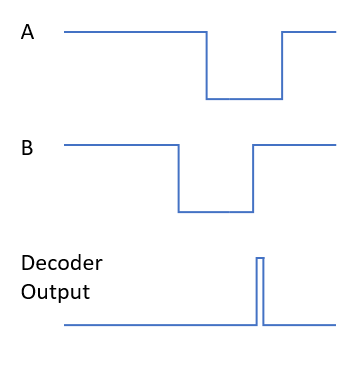
\includegraphics[width=0.4\textwidth]{{data/RotaryCCWDecoder.png}}
	\caption{Output of rotary decoder, counterclockwise turn.} 
	\label{RotaryDecoderDiagram}    
\end{fullfigure}
The switch input and the two out-of-phase signals from each rotary encoder are decoded with the rotary controller. The rotary logic block consists of a debouncer for the push button and a decoder for the rotary encoder. 

The debouncer (Figure~\ref{Block:RotaryDebouncer}) takes as inputs the active-low button input (Rotary1\_P and Rotary2\_P on the schematic), clock, and active-low reset signal. It outputs a single active-high clock pulse whenever the button input signal is low for longer than 100000 clocks, which was chosen through testing the switches. 

The decoder (Figure~\ref{Block:RotaryDecoder}) takes as inputs the two active-low outputs from the encoder (Rotary1\_A and Rotary1\_B, and Rotary2\_A and Rotary2\_B on the schematic), and the reset and clock signals, and outputs a single active-high clock pulse for each counter-clockwise turn of the rotary encoder, where output A leads B (Figure~\ref{RotaryDecoderDiagram}). 

This is accomplished by first debouncing the input using a counter and comparator to eliminate glitches. Several DFFs are used in series in order to read inputs A and B from two consecutive clocks to determine when edges have occurred. An SRFF is set low when input B goes from low to high while input A is still low, and is set high otherwise. The inverse of this is returned as the output, resulting in a decoder for one direction. Two decoders are used for each rotary encoder to distinguish clockwise and counterclockwise turns (Figure~\ref{Block:Rotary}). 

\subsubsection{VRAM and LCD}\index{VRAM}\index{LCD} \label{subsec:VRAMLCD}
\begin{fullfigure} 
	\centering
	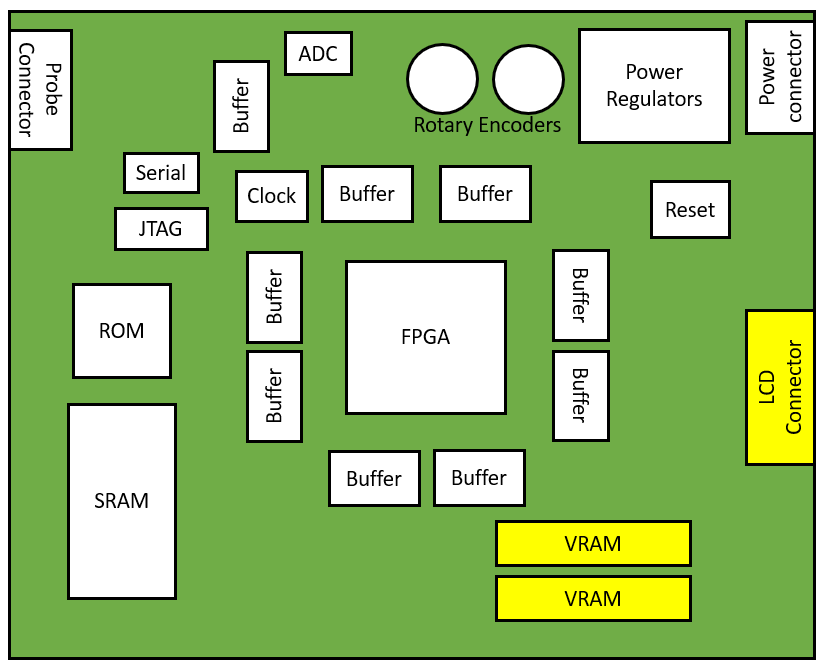
\includegraphics[width=1\textwidth]{{data/Board_Layout_Display.png}}
	\caption{Board Layout: Display.} 
	\label{Layout:Display}    
\end{fullfigure}

\begin{fullfigure} 
	\centering
	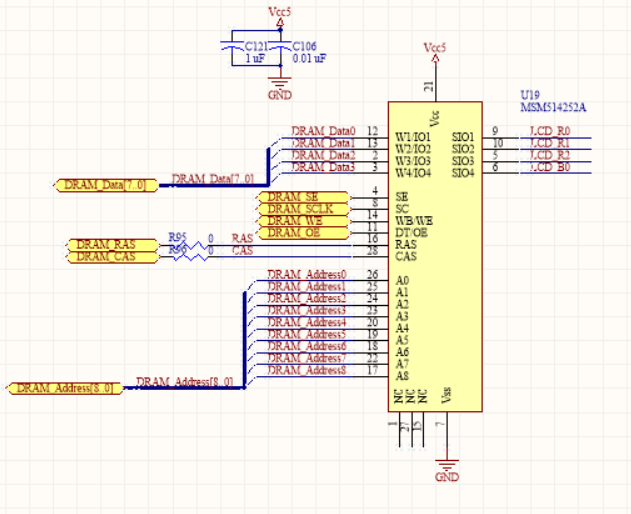
\includegraphics[width=0.7\textwidth]{{data/VRAM_1.png}}
	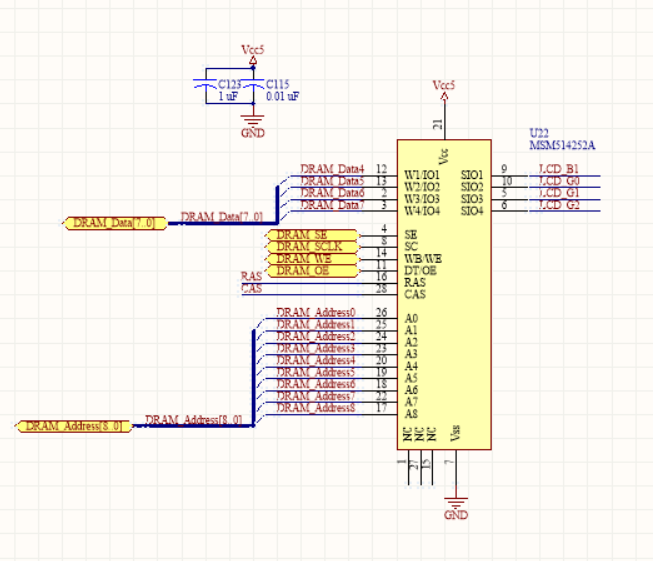
\includegraphics[width=0.7\textwidth]{{data/VRAM_2.png}}
	\caption{VRAM schematics.} 
	\label{Schematics:VRAM}    
\end{fullfigure}

\begin{fullfigure} 
	\centering
	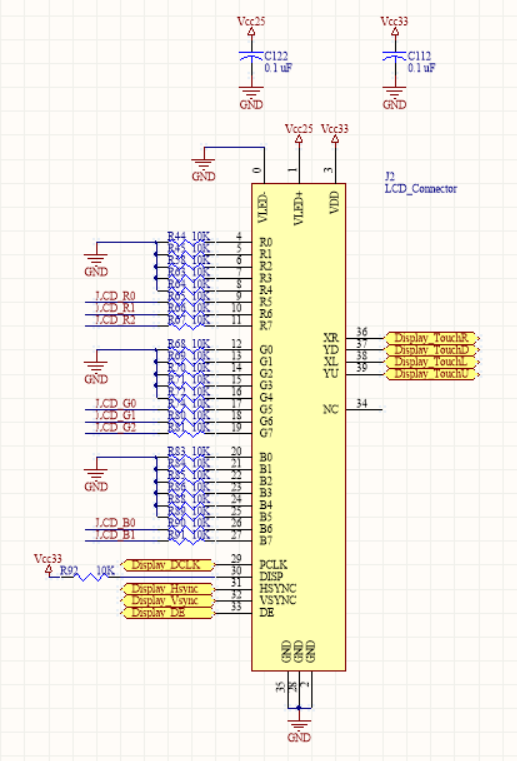
\includegraphics[width=0.8\textwidth]{{data/LCD_Connector.png}}
	\caption{LCD connector schematics.} 
	\label{Schematics:LCD}    
\end{fullfigure}

% summary 
Two 256Kx4 DRAM with 512x4 SAM (Serial Access Memory) chips (U19, U22, MT42C4225) were used for a total of 8 bits of data, with a 480x272 RGB TFT LCD (Connector J2, ER-TFT043-3).

%TODO vram lines
\marginlabel{VRAM:} \index{VRAM}
Each VRAM sends 4 bits of serial data to the LCD, and receives 4 bits of data from the CPU, along with a 9 bit address bus, row address strobe (RAS), column address strobe (CAS), write enable (WE), and output enable (OE) signals from the VRAM controller.  A serial clock signal is also sent to the VRAM. The LCD controller generates the various clock signals that are sent to synchronize the VRAM and LCD. 
The same address bus and control signals are used between the two VRAM, and each sends and receives 4 different data bits. 

Resistors R95 and R96 are included in series in the RAS and CAS lines for termination.

The VRAM consists of the DRAM, transfer circuitry, and SAM. Read and write cycles are performed to read and write to the DRAM, and read transfer cycles are performed to transfer a row from the DRAM to SAM. 
Serial output cycles are performed to output the current row data from the SAM to the LCD. The VRAM is refreshed when no other operations are being performed in order to retain data. 

\marginlabel{LCD:} \index{LCD}
The LCD receives 8 bits of data in parallel from the VRAM: 3 bits red, 3 bits green, and 2 bits blue, with the unused color bits pulled down. It also receives a horizontal sync, vertical sync, clock, and data enable signal from the LCD controller. The touch inputs were unused. 

The LCD also required a 25V backlight supply (VLED on the schematic). A step-up converter (U21) was used, which is discussed in more detail in Section~\ref{subsec:Power}.  

\marginlabel{Logic overview:}
The VRAM-LCD system consists of a VRAM controller and LCD controller that interact with each other, the CPU, and the VRAM and LCD.

\begin{fullfigure} 
	\centering
	\includegraphics[width=1\textwidth]{{data/VRAM_LCD_Block.png}}
	\caption{Block Diagram for VRAM and LCD.}
	\label{Block:VRAM_LCD}    
\end{fullfigure}

\begin{fullfigure} 
	\centering
	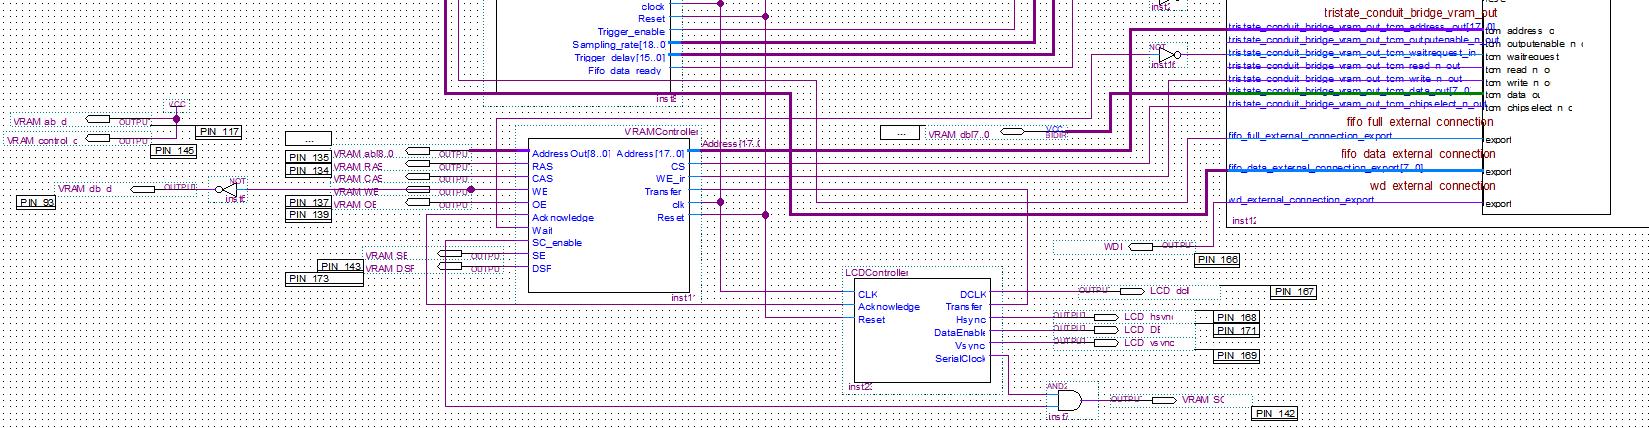
\includegraphics[width=1\textwidth]{{data/VRAMCPU.png}}
	\caption{VRAM and LCD Controllers.}
	\label{Block:VRAM_CPU}    
\end{fullfigure}

\marginlabel{VRAM Controller:} \index{VRAM! Controller}
The VRAM controller takes several inputs from the CPU: 1-bit chip select and write enable signals, and an 18-bit address. It also takes as an input a transfer request signal from the display controller. A state machine is used to generate the output signals, the RAS, CAS, address selector, WE, OE, serial clock, CPU wait output, and transfer acknowledge signals.

\begin{fullfigure} 
	\centering
	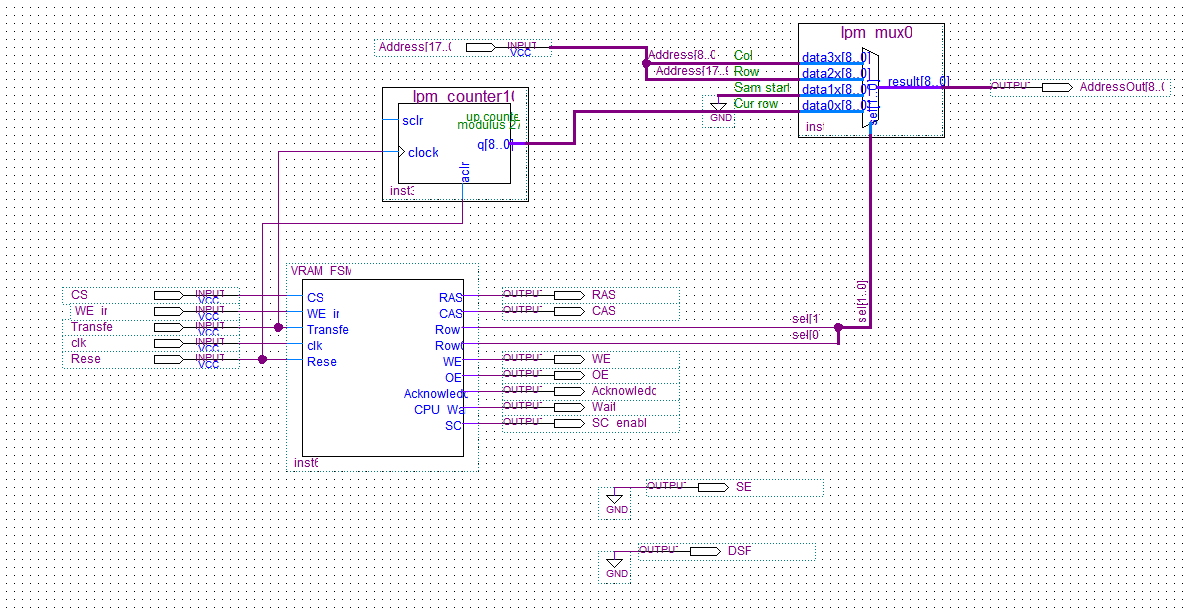
\includegraphics[width=1\textwidth]{{data/VRAM_Controller.png}}
	\caption{VRAM Controller.}
	\label{Block:VRAM_Controller}    
\end{fullfigure}

%mux address 
\marginlabel{Address:} The output address is selected and outputted using a multiplexer. For either the column or row address, the first or second half of the input address is returned. In the case of a row transfer, the SAM start address, 0 for the beginning of the memory, and the current row, are outputted at the appropriate times. A counter is used to increment the current row for after each row transfer cycle, from row 0 to 272, or the total height of the LCD. 
%TODO memory map

%State machine 
\marginlabel{VRAM State Machine:} The read, write, row transfer, and refresh cycles are performed with a Moore state machine, Appendix~\ref{AP:VRAM_FSM.vhd}. 

The state machine begins at an idle state, and goes back to the idle state after each cycle is completed. If there is a row transfer request, when the transfer flag is active, the row transfer cycle is performed. If there is a write request, when the chip select and write enable inputs are active, then the write cycle is performed. If there is a read select, when the chip select is enabled but write enable is not, then the read cycle is performed. If none of these cycles are to be completed when in the idle state, a refresh cycle is performed. 

Timing diagrams were used to create the state machine with the correct outputs, found in Appendix~\ref{AP:Timing}.

\marginlabel{LCD Controller:} \index{LCD! Controller}
The LCD controller is used to generate the clock signals for the LCD. 

The Vertical Sync (VSYNC) signal is used for changing rows, and Horizontal Sync (HSYNC) for changing columns. The Data Enable (DE) signal is also generated for when input data is valid within the VSYNC AND HSYNC signals. A 12 MHz clock signal is also sent to the LCD, while a serial clock signal is generated  for the VRAM clock input to the serial address counter for the SAM registers.

The row transfer request (Transfer signal in Figure~\ref{Block:LCD_Controller}) is set when the end of the row has been reached, and the flag is cleared once the VRAM controller has completed the row transfer and set the transfer acknowledge flag. %todo unsure

The timing diagrams can be found in Appendix~\ref{AP:Timing}, Figures~\ref{AP:LCD_Horizontal_Timing} and \ref{AP:LCD_Vertical_Timing}.

\begin{fullfigure} 
	\centering
	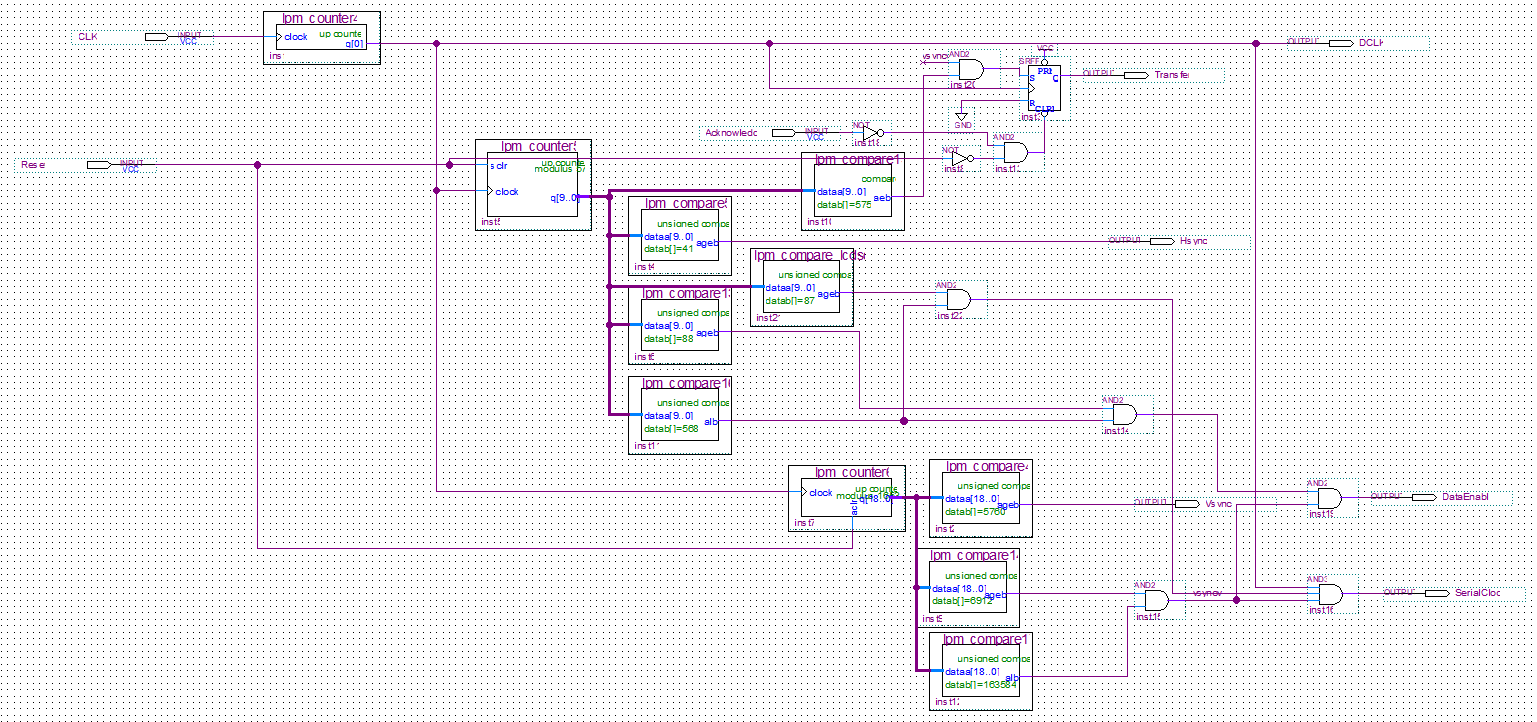
\includegraphics[width=1\textwidth]{{data/LCD_Controller.png}}
	\caption{LCD Controller, with comparators for defining valid regions in the signals.}
	\label{Block:LCD_Controller}    
\end{fullfigure}

\subsubsection{JTAG, Reset, and Clock} 
% separate? 
\begin{fullfigure} 
	\centering
	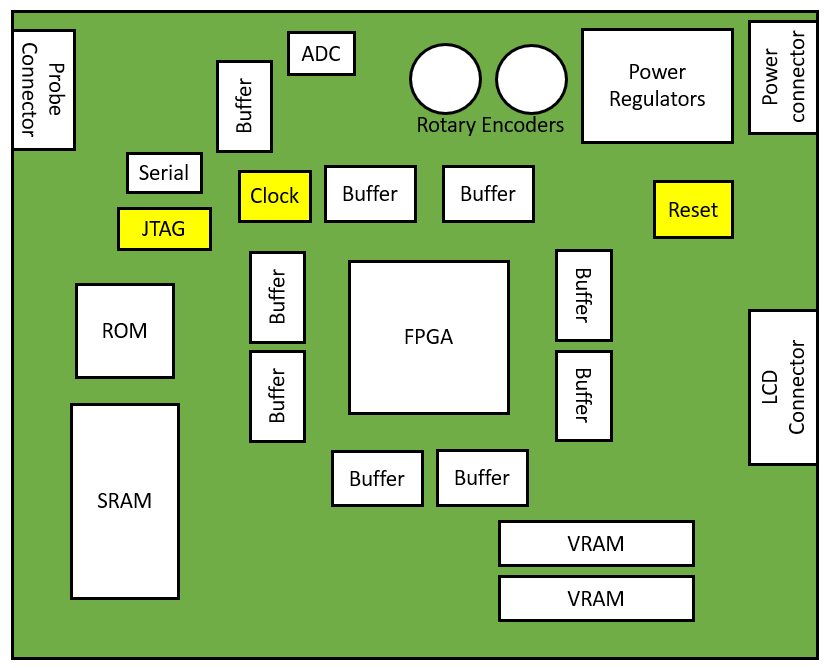
\includegraphics[width=1\textwidth]{{data/Board_Layout_FPGAothers.png}}
	\caption{Board Layout: Clock, JTAG, Reset.} 
	\label{Layout:FPGAothers}    
\end{fullfigure}

\marginlabel{JTAG:} \index{JTAG}
\begin{fullfigure} 
	\centering
	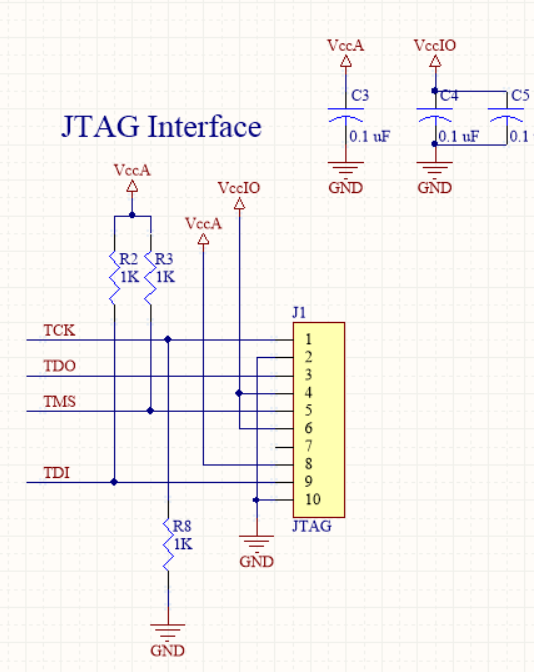
\includegraphics[width=0.6\textwidth]{{data/JTAG.png}}
	\caption{JTAG interface Schematic.}
	\label{Schematic:JTAG}    
\end{fullfigure}
A JTAG interface was used for debugging the system, seen in Figure~\ref{Schematic:JTAG} and is connected directly to the appropriate FPGA pins. 

\marginlabel{Reset:} \index{Reset}
\begin{fullfigure} 
	\centering
	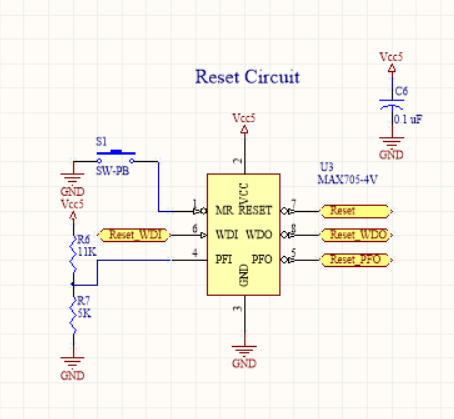
\includegraphics[width=0.6\textwidth]{{data/ResetCircuit.png}}
	\caption{Reset Circuit Schematic.}
	\label{Schematic:Reset}    
\end{fullfigure}

A reset circuit is used, which includes a microprocessor supervisory device (U3, MAX705).
The watchdog input (WDI) is implemented in the main loop, and a voltage divider is used for a power-fail warning at 4 V from the 5 V supply. 

The active-low watchdog output, power-fail output, and reset output, and manual reset output are combined for an overall reset signal that is sent to the CPU and various controllers. 

\marginlabel{Clock:} \index{Clock}
\begin{fullfigure} 
	\centering
	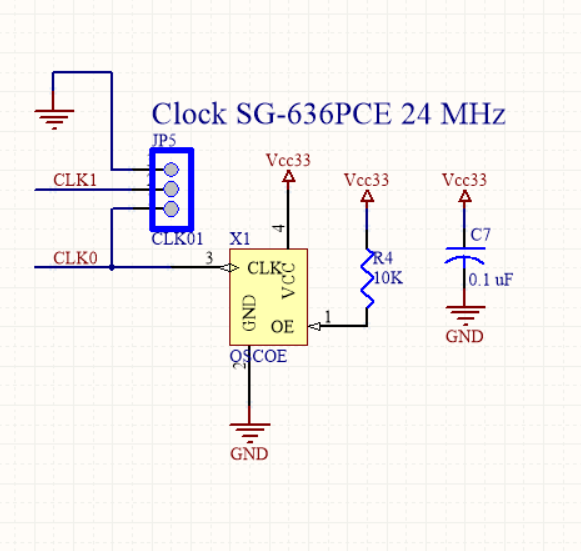
\includegraphics[width=0.6\textwidth]{{data/Clock.png}}
	\caption{Clock Circuit Schematic.}
	\label{Schematic:Clock}    
\end{fullfigure}
A 24 MHz oscillator (X1) was used for the clock input for the device, with the CLK0 signal connected directly to the appropriate FPGA pin. 

\subsubsection{Fixes} %TODO
wrong adc footprint, buffer soldering error, backwards LCD connector footprint

%%%%%%%%%%%%%%%%%%%%%%%%%%%%%%%%%%%%%%%%%%%%%%%%%%%%%%%%%%%%% Software
\subsection{Software} \index{Software} \label{subsec:software}

\subsubsection{Software System Overview} 

\begin{fullfigure} 
	\centering
	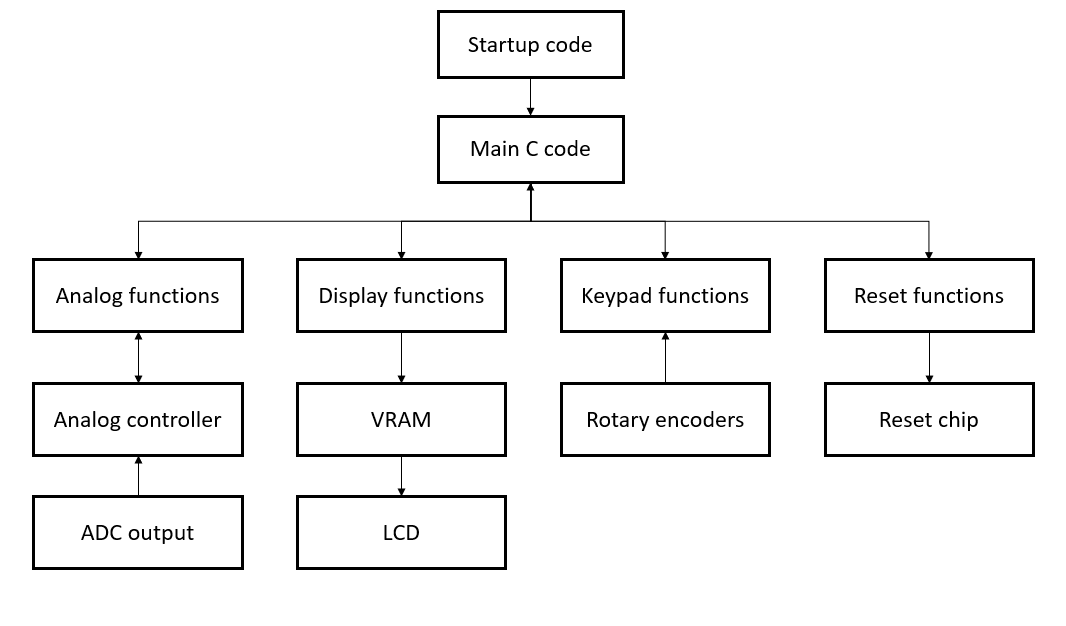
\includegraphics[width=1\textwidth]{{data/software/Main_Block_Software.png}}
	\caption{Software block diagram overview.}
	\label{Block:Software}    
\end{fullfigure}
The main components that were written were routines for the analog settings, display, and keypad \footnote{rotary encoders were implemented instead of a keypad, so references to the keypad refer to the rotary encoders}. As shown in Figure~\ref{Block:Software}, the main code handles the main loop and calls the various utility functions. The analog functions set the trigger settings used by the analog controller, and also clock out the signal data from the FIFO buffer into a buffer in the data section to be displayed. Display functions clear the display and plot a pixel by writing to the VRAM, whose data is outputted to the LCD. Keypad routines include an event handler and getting the key pressed. A reset function that toggles the watchdog input on the reset chip was also written. These will be discussed in more details below. 

\subsubsection{Analog Software} \label{subsec:AnalogSoftware} \index{Analog! Software}

\begin{fullfigure} 
	\centering
	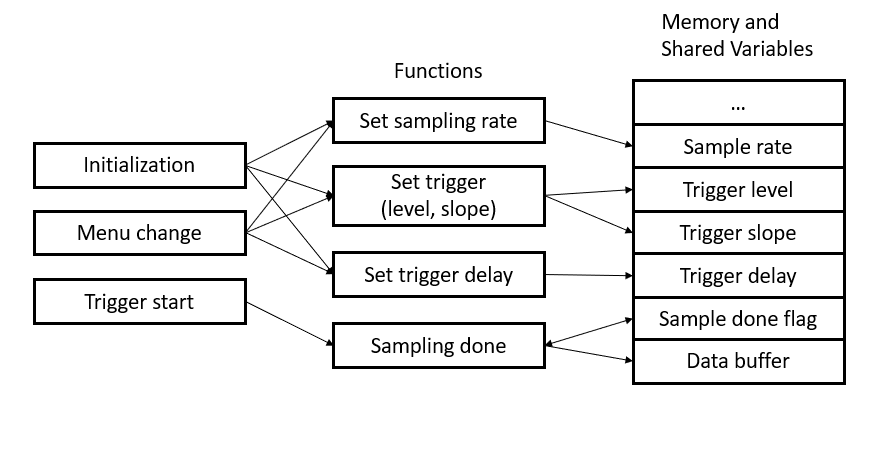
\includegraphics[width=1\textwidth]{{data/software/Analog_Block_Software.png}}
	\caption{Analog software block diagram.}
	\label{Block:AnalogSoftware}    
\end{fullfigure}
The analog software includes analog  initialization, which sets the trigger enable and sample done flags to false, as well as a start\_sample initialization for to start the sample. It enables triggering, sets autotriggering, and sets the sample done flag to false. The sample done flag is used to ensure that only one sample is taken per enabled trigger.

Sampling\_done checks to see if the buffer is full and a sample has been taken. If it is, and no sample has been taken yet, the data from the FIFO is clocked out and stored in the data buffer shared variable to be displayed. These functions are called by the main loop and the various trace and sampling utilities. 

There are also functions for setting the sampling rate, trigger level, trigger slope, and trigger delay. These are called upon initialization and when their corresponding settings have been changed from the menu. These directly change the outputs that are sent to the analog controller and are used to take the sample.  

\begin{fullpage}\label{Code:analog.S}
\lstinputlisting[style=AS]{../osc134/analog.S} 
\end{fullpage}

\subsubsection{Display Software} \label{subsec:DisplaySoftware} \index{Display! Software}

\begin{fullfigure} 
	\centering
	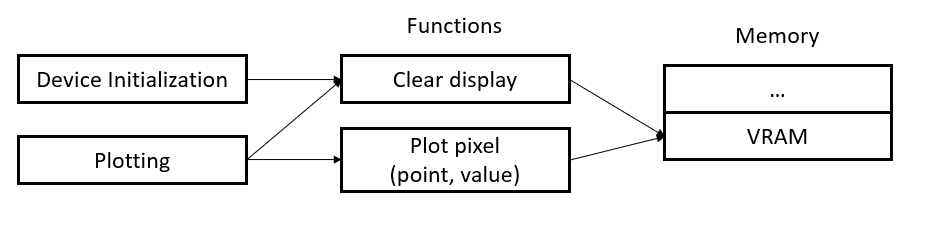
\includegraphics[width=1\textwidth]{{data/software/Display_Block_Software.png}}
	\caption{Display software block diagram.}
	\label{Block:DisplaySoftware}    
\end{fullfigure}

The display functions perform the basic requirements of clearing the LCD, or turning all the pixels black, and plotting a specified pixel on the display. These modify the data at the appropriate addresses in the VRAM. These functions are used upon initialization and when plotting the menu and sample, as the display is cleared between each sample. 

\begin{fullpage}\label{Code:display.S}
	\lstinputlisting[style=AS]{../osc134/displayFunc.S} 
\end{fullpage}

\subsubsection{Keypad Software} \label{subsec:KeypadSoftware} \index{Keypad! Software}

\begin{fullfigure} 
	\centering
	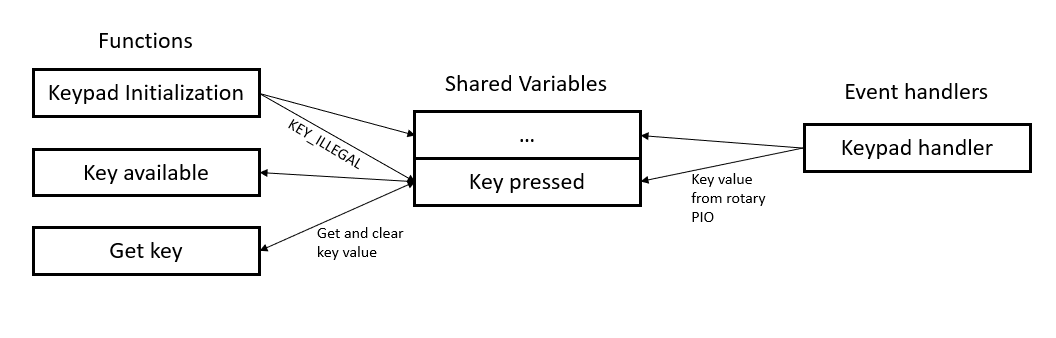
\includegraphics[width=1\textwidth]{{data/software/Key_Block_Software.png}}
	\caption{Keypad software block diagram.}
	\label{Block:KeypadSoftware}    
\end{fullfigure}

The keypad software has an event handler for whenever a key is pressed and a keypad interrupt occurs. The key value is stored in the key\_pressed shared variable. This is accessed by the key\_available and getKey functions. Key\_available returns whether or not there is a valid key, and if there is, getKey is called and will return the valid key. These are called from the main loop when checking if there is keypad input. 

\begin{fullpage}\label{Code:keypad.S}
	\lstinputlisting[style=AS]{../osc134/keypad.S} 
\end{fullpage}


\subsubsection{Watchdog Reset} \label{subsec:ResetSoftware}
A reset function to toggle the watchdog input on the reset circuit (Reset\_WDI, Figure~\ref{Schematic:Reset}) was also written. The toggled output is sent out to the reset device. This function is called in the main loop (Listing ~\ref{Code:mainloop.c}), which should never stall or take greater than the time required for the reset device to send out a watchdog reset signal. If it does, some error has occurred and the system will reset. 

\begin{fullpage}\label{Code:reset.S}  
	\lstinputlisting[style=AS]{../osc134/reset.S} 
\end{fullpage}

\subsubsection{Header files} \label{subsec:Headers}

\begin{fullpage}\label{Code:general.h}
	\lstinputlisting[style=AS]{../osc134/general.h} 
\end{fullpage}

The rest of the code used can be found at Appendix~\ref{AP:Code}.

%%%%%%%%%%%%%%%%%%%%%%%%%%%%%%%%%%%%%%%%%%%%%%%%%%%%%%%%%%%%% Appendix
\appendix \index{Appendix}
\section{Timing Diagrams} \label{AP:Timing} \index{Timing}
\subsection{ADC}
	\begin{fullfigure} 
		\centering
		\includegraphics[width=1\textwidth]{{data/timing/ADC.png}}
		\caption{ADC Timing Diagram}
		\label{AP:ADC_Timing}    
	\end{fullfigure}

\subsection{LCD}
\begin{fullfigure} 
	\centering
	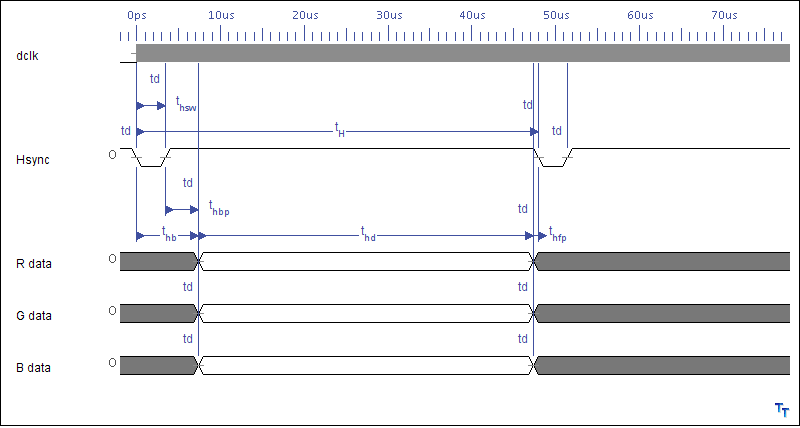
\includegraphics[width=1\textwidth]{{data/timing/LCD_Horizontal.png}}
	\caption{LCD Horizontal Timing Diagram}
	\label{AP:LCD_Horizontal_Timing}    
\end{fullfigure}

\begin{fullfigure} 
	\centering
	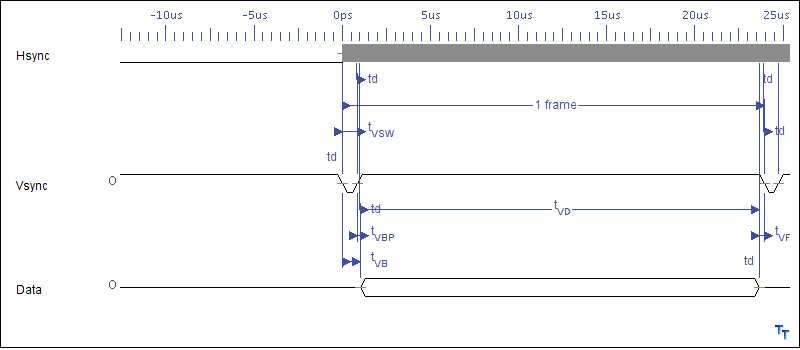
\includegraphics[width=1\textwidth]{{data/timing/LCD_Vertical.png}}
	\caption{LCD Vertical Timing Diagram}
	\label{AP:LCD_Vertical_Timing}    
\end{fullfigure}

\subsection{ROM and RAM}
\begin{fullfigure} 
	\centering
	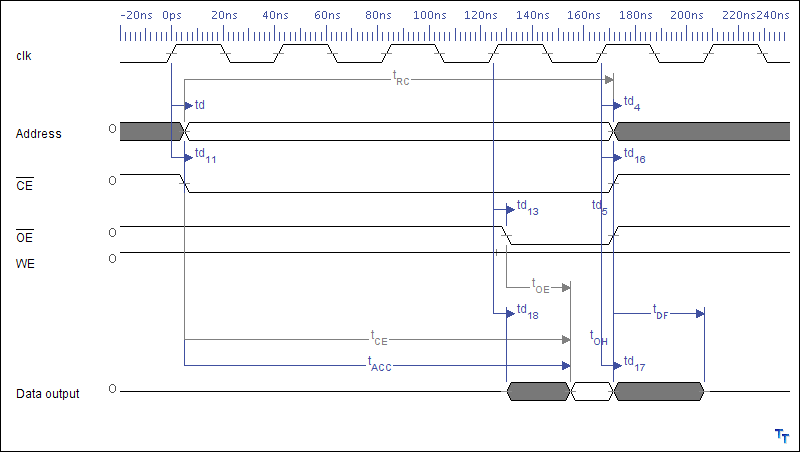
\includegraphics[width=1\textwidth]{{data/timing/ROM_Read.png}}
	\caption{ROM Read Cycle Diagram}
	\label{AP:ROM_Read_Timing}    
\end{fullfigure}

\begin{fullfigure} 
	\centering
	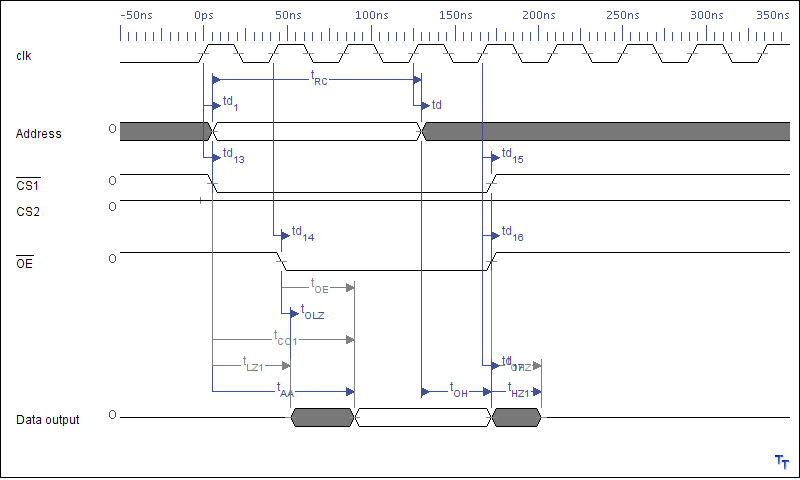
\includegraphics[width=1\textwidth]{{data/timing/SRAM_Read.png}}
	\caption{RAM Read Cycle Diagram}
	\label{AP:RAM_Read_Timing}    
\end{fullfigure}

\begin{fullfigure} 
	\centering
	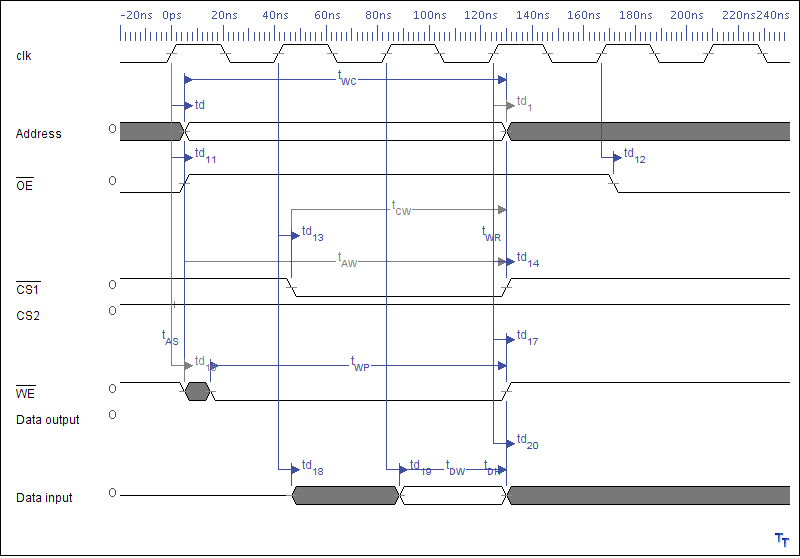
\includegraphics[width=1\textwidth]{{data/timing/SRAM_Write.png}}
	\caption{RAM Write Cycle Diagram}
	\label{AP:RAM_Write_Timing}    
\end{fullfigure}

\subsection{VRAM}
\begin{fullfigure} 
	\centering
	\includegraphics[width=1\textwidth]{{data/timing/VRAM_Read_MT.png}}
	\caption{VRAM Read Cycle Diagram}
	\label{AP:VRAM_Read_Timing}    
\end{fullfigure}

\begin{fullfigure} 
	\centering
	\includegraphics[width=1\textwidth]{{data/timing/VRAM_Write_MT.png}}
	\caption{VRAM Write Cycle Diagram}
	\label{AP:VRAM_Write_Timing}    
\end{fullfigure}

\begin{fullfigure} 
	\centering
	\includegraphics[width=0.75\textwidth]{{data/timing/VRAM_Read_Transfer_MT.png}}
	\caption{VRAM Row Transfer Cycle Diagram}
	\label{AP:VRAM_Transfer_Timing}    
\end{fullfigure}

\begin{fullfigure} 
	\centering
	\includegraphics[width=1\textwidth]{{data/timing/VRAM_refresh_MT.png}}
	\caption{VRAM Refresh Cycle Diagram (CAS before RAS)}
	\label{AP:VRAM_Refresh_Timing}    
\end{fullfigure}

\begin{fullfigure} 
	\centering
	\includegraphics[width=1\textwidth]{{data/timing/VRAM_Serial_Write_MT.png}}
	\caption{VRAM Serial Write Cycle Diagram}
	\label{AP:VRAM_Serial_Write_Timing}    
\end{fullfigure}

\section{Device Images}
\begin{fullfigure} 
	\centering
	\includegraphics[width=1\textwidth]{{data/Scope_Front}}
	\caption{Front of device}
	\label{Scope:front}    
\end{fullfigure}

\begin{fullfigure} 
	\centering
	\includegraphics[width=1\textwidth]{{data/Scope_Back}}
	\caption{Back of device}
	\label{Scope:back}    
\end{fullfigure}

\begin{fullfigure} 
	\centering
	\includegraphics[width=1\textwidth]{{data/Scope_On}}
	\caption{Device running with sinusoidal input} %where is the caption consistency
	\label{Scope:sine}    
\end{fullfigure}

\section{Schematics and PCB} \label{AP:Schematics} \label{AP:PCB} \index{Schematics} \index{PCB}

% entire schematic and pcb

\includepdf[pages={-}, fitpaper=true]{data/Schematics.pdf} 
 
% list of changes to pcb and glen's code 
%TODO

\section{Software} \label{AP:Software} \index{Code}

\subsection{Hardware descriptions} \label{AP:VHDL}
\begin{fullpage}
	\label{AP:scopetrig.vhd} 
	\lstinputlisting[style=VHDLMeUp2]{data/scoptrig.vhd} 
	
	\label{AP:VRAM_FSM.vhd}
	\lstinputlisting[style=VHDLMeUp2]{data/VRAM_FSM.vhd}
\end{fullpage}

\subsection{Main code} \label{AP:Code} \index{Code}
\begin{fullpage}
	
	\label{Code:mainloop.c}
	\lstinputlisting[style=C]{../osc134/mainloop.c}
	
	\label{Code:scopedef.h}
	\lstinputlisting[style=C]{../osc134/scopedef.h}
	
	\label{Code:interfac.h}
	\lstinputlisting[style=C]{../osc134/interfac.h} 
	
	\label{Code:menu.c}
	\lstinputlisting[style=C]{../osc134/menu.c}
	
	\label{Code:menu.h}
	\lstinputlisting[style=C]{../osc134/menu.h}
	
	\label{Code:menuact.c}
	\lstinputlisting[style=C]{../osc134/menuact.c}  
	
	\label{Code:menuact.h}
	\lstinputlisting[style=C]{../osc134/menuact.h} 
	
	\label{Code:keyproc.c}
	\lstinputlisting[style=C]{../osc134/keyproc.c}
	
	\label{Code:keyproc.h}
	\lstinputlisting[style=C]{../osc134/keyproc.h}  
	
	\label{Code:lcdout.c}
	\lstinputlisting[style=C]{../osc134/lcdout.c}
	
	\label{Code:lcdout.h}
	\lstinputlisting[style=C]{../osc134/lcdout.h}
	
	\label{Code:tracutil.c}
	\lstinputlisting[style=C]{../osc134/tracutil.c}
	
	\label{Code:tracutil.h}
	\lstinputlisting[style=C]{../osc134/tracutil.h}  
		
	\label{Code:char57.c}
	\lstinputlisting[style=C]{../osc134/char57.c}     
\end{fullpage}

\printindex 
\end{document}


\begin{comment}

\begin{description}

\item[Line spacing]\index{line spacing}

\end{description}

\attention

\footnote{text}

\index{}\marginlabel{}

\texttt{}

\begin{figure} [H]
\centering
\includegraphics[width=0.75\textwidth]{{data/}}
\caption{block diagram}
\label{LCDBlockDiagram}    
\end{figure}

\includepdf[pages={1}]{myfile.pdf} 
pages={-} 
for all 
\end{comment}